\nonstopmode
%%*****************************************************************************
%% $Id: extex-users.tex 5326 2007-02-27 13:09:26Z gene $
%%*****************************************************************************
%% Author: Gerd Neugebauer
%%-----------------------------------------------------------------------------
\documentclass{texinputs/extex-doc}

\newif\ifdraft\drafttrue
\def\Version{0.1}
\title{Reference Manual}
\author{Gerd Neugebauer}

\usepackage{texinputs/dirlist}
\usepackage{texinputs/iconmargin}
\usepackage{makeidx}

\newcommand\Arg[1]{\(\langle\){\tt\itshape #1}\(\rangle\)}
\newcommand\CLI[1]{\texttt{-#1}\index{#1@\texttt{-#1}}}
\newcommand\Property[1]{\texttt{#1}\index{#1@\texttt{#1}}}
\newcommand\File[1]{\texttt{#1}\index{#1@\textsf{#1}}}
\newcommand\Prog[1]{\texttt{#1}\index{#1}}
\newcommand\Mode[1]{\texttt{#1}\index{#1}}
\newcommand\macro[1]{\texttt{\char`\\ #1}\index{#1@\texttt{\char`\\ #1}}}
\newcommand\Macro[1]{\texttt{\char`\\ #1}}
\newcommand\tag[1]{%
    \(\langle\)\textit{#1}\(\rangle\)%
    \index{#1@\protect\Tag{#1}}}
\newcommand\Tag[1]{\texorpdfstring{%
    \(\langle\)\textit{#1}\(\rangle\)}{<#1>}}

\newenvironment{syntax}{%
  \begin{tabbing}\kern2em\=\kern2em\=\kill
  }{%
  \end{tabbing}}
\newcommand\SyntaxDef{\>\(\rightarrow\)\>}
\newcommand\SyntaxOr{\>\(|\)\>}

\def\n{\char`\\n}
\def\t{\char`\\t}

\providecommand\BibTeX{Bib\TeX}

\makeindex

\begin{document}%%%%%%%%%%%%%%%%%%%%%%%%%%%%%%%%%%%%%%%%%%%%%%%%%%%%%%%%%%%%%%%

\begin{titlepage}
  \parindent=0pt
  \begin{center}
  \vspace*{1pt}
  \vfill
  \ExBibbox
  \vfill
  \textsf{\bfseries\Huge \csname@title\endcsname}
  \vfill
  \textsf{\Large Version \Version}
  \vfill
  \textsf{\large \csname@author\endcsname}
  \vfill
  \vfill
%\maketitle

  \begin{abstract}\parindent=0pt
    This document describes \ExBib. It explains how to get \ExBib\ up
    and running and which features \ExBib\ offers to you.

    The intended audience for this document are end users of a
    bibliography processor who want to use \ExBib\ on the command line or
    as plug-in replacement of \BibTeX.
  \end{abstract}
  \ifdraft
  \unitlength=1mm
  \begin{picture}(0,0)
    \put(51,98.5){\makebox(0,0){%
        \scalebox{6}{%
          \rotatebox{45}{%
            \color{black}\textsf{\Huge\bfseries Draft}}}}}
    \put(50,98){\makebox(0,0){%
        \scalebox{6}{%
          \rotatebox{45}{%
            \color{red}\textsf{\Huge\bfseries Draft}}}}}
  \end{picture}
  \fi
  \end{center}
\newpage
\footnotesize
\copyright\ 2008 The \ExTeX\ Group and individual authors listed below 
\medskip

Permission is granted to copy, distribute and/or modify this document
under the terms of the GNU Free Documentation License, Version 1.2 or
any later version published by the Free Software Foundation. A copy of
the license is included in the section entitled ``GNU Free
Documentation License''.
\bigskip

This product includes software developed by the Apache Software
Foundation (http://www.apache.org/).

\vfill

Gerd Neugebauer\\
Im Lerchelsb\"ohl 5\\
64521 Gro\ss-Gerau (Germany)
\smallskip

\href{mailto://gene@gerd-neugebauer.de}{gene@gerd-neugebauer.de}

\end{titlepage}

\tableofcontents

%------------------------------------------------------------------------------

%%*****************************************************************************
%% Copyright (c) 2008 Gerd Neugebauer
%%
%% Permission is granted to copy, distribute and/or modify this document
%% under the terms of the GNU Free Documentation License, Version 1.2
%% or any later version published by the Free Software Foundation;
%% with no Invariant Sections, no Front-Cover Texts, and no Back-Cover Texts.
%%
%%*****************************************************************************
%% $Id:intro.tex 7067 2008-05-18 11:06:56Z gene $
%%*****************************************************************************
%% Author: Gerd Neugebauer
%%-----------------------------------------------------------------------------

\chapter{Introduction}
%@author Gerd Neugebauer

\ExTeX\index{ExTeX@\ExTeX} aims at providing a high-quality
typesetting system. The development of \ExTeX\ has been inspired by
the experiences with \TeX\ \cite{knuth:texbook}. The focus lies on an
open design and a high degree of configurability.

A tight integration of several components is one of the possibilities
opened by \ExTeX. To work into this direction \ExBib\ has been
implemented. It is a plug-in replacement for
\BibTeX~0.99c\index{BibTeX 0.99c@\BibTeX~0.99c}\cite{btxdoc,btxhak}
or \BibTeX~8\index{BibTeX 8@\BibTeX~8}.

\begin{figure}[hb]
  \centering
  %%*****************************************************************************
%% $Id$
%%*****************************************************************************
%% Author: Gerd Neugebauer
%%-----------------------------------------------------------------------------
\begingroup\small
\def\processor(#1)#2{%
  \begin{scope}[shift={(#1)}]
    \draw[thick,color=white!80!gray,fill==white!70!gray]
    (1,-0.5) rectangle (9,4.5);
    \shade[top color=white!90!green,bottom color=white!60!green,draw=green!40!black,thick]
    (0.5,0) rectangle (8.5,5);
    \draw (4.5,2.5) node{#2};
    \shade[top color=white!90!green,bottom color=white!60!green,draw=green!40!black,thick]
    (0,1) rectangle (1,2);
    \shade[top color=white!90!green,bottom color=white!60!green,draw=green!40!black,thick]
    (0,3) rectangle (1,4);
  \end{scope}
}
\def\data(#1)#2{%
  \begin{scope}[shift={(#1)}]
    \draw[thick,color=white!80!gray,fill==white!70!gray]
    (0.3,-.3) -- (5.3,-.3) -- (5.3,1.7) -- (4.3,2.7) -- (0.3,2.7) -- cycle;
    \shade[top color=white!90!yellow,bottom color=white!60!yellow,draw=red!40!black,thick]
    (0,0) -- (5,0) -- (5,2) -- (4,3) -- (0,3) -- cycle;
    \draw (2.5,1.5) node{#2};
  \end{scope}
}
\def\datas(#1)#2{%
  \begin{scope}[shift={(#1)}]
    \draw[thick,color=white!80!gray,fill==white!70!gray]
    (0.3,-.3) -- (5.3,-.3) -- (5.3,1.7) -- (4.3,2.7) -- (0.3,2.7) -- cycle;
    \begin{scope}[shift={(.15,.15)}]
      \draw[thick,color=white!80!gray,fill==white!70!gray]
      (0.3,-.3) -- (5.3,-.3) -- (5.3,1.7) -- (4.3,2.7) -- (0.3,2.7) -- cycle;
    \end{scope}
    \begin{scope}[shift={(.1,.1)}]
      \draw[thick,color=white!80!gray,fill==white!70!gray]
      (0.3,-.3) -- (5.3,-.3) -- (5.3,1.7) -- (4.3,2.7) -- (0.3,2.7) -- cycle;
    \end{scope}
    \begin{scope}[shift={(.05,.05)}]
      \draw[thick,color=white!80!gray,fill==white!70!gray]
      (0.3,-.3) -- (5.3,-.3) -- (5.3,1.7) -- (4.3,2.7) -- (0.3,2.7) -- cycle;
    \end{scope}
    \begin{scope}[shift={(.3,.3)}]
      \shade[top color=white!90!yellow,bottom color=white!60!yellow,draw=red!40!black,thick]
      (0,0) -- (5,0) -- (5,2) -- (4,3) -- (0,3) -- cycle;
    \end{scope}
    \begin{scope}[shift={(.2,.2)}]
      \shade[top color=white!90!yellow,bottom color=white!60!yellow,draw=red!40!black,thick]
      (0,0) -- (5,0) -- (5,2) -- (4,3) -- (0,3) -- cycle;
    \end{scope}
    \begin{scope}[shift={(.1,.1)}]
      \shade[top color=white!90!yellow,bottom color=white!60!yellow,draw=red!40!black,thick]
      (0,0) -- (5,0) -- (5,2) -- (4,3) -- (0,3) -- cycle;
    \end{scope}
    \shade[top color=white!90!yellow,bottom color=white!60!yellow,draw=red!40!black,thick]
    (0,0) -- (5,0) -- (5,2) -- (4,3) -- (0,3) -- cycle;
    \draw (2.5,1.5) node{#2};
  \end{scope}
}
\def\arrow(#1)#2#3{%
  \begin{scope}[shift={(#1)}#3,scale=.5]
    \begin{scope}[shift={(#2)}]
      \draw[thick,color=white!80!gray,fill==white!70!gray]
      (0,1) -- (5,1) -- (5,0) -- (6,2) -- (5,4) -- (5,3) -- (0,3) -- cycle;
    \end{scope}
    \shade[top color=white!90!gray,bottom color=white!60!gray,draw=gray!40!black,thick]
    (0,1) -- (5,1) -- (5,0) -- (6,2) -- (5,4) -- (5,3) -- (0,3) -- cycle;
  \end{scope}
}
%
\begin{tikzpicture}[scale=.35]\sf
  \processor(10,30){Text Processor}

  \arrow(10.5,29){.3,.3}{,rotate=270}
  \datas(9,22){file.aux}
  \arrow(10.5,21){.3,.3}{,rotate=270}

  \processor(10,12){\ExBib}
  \arrow(19.5,13.5){.3,-.3}{}
  \data(23.5,13){file.blg}

  \arrow(18.5,18){-.3,-.3}{,rotate=90}
  \data(15,22){file.bbl}
  \arrow(18.5,26){-.3,-.3}{,rotate=90}

  \arrow(6,13.5){.3,-.3}{}
  \datas(0,13){*.bib}

  \arrow(12.5,8){-.3,-.3}{,rotate=90}
  \datas(9,4){*.bst}

  \arrow(18.5,8){-.3,-.3}{,rotate=90}
  \data(15,4){*.csf}

  \arrow(23,10){-.3,-.3}{,rotate=135}
  \datas(21,5){Config}

\end{tikzpicture}
\endgroup
\endinput
%
% Local Variables: 
% mode: latex
% TeX-master: nil
% End: 

  \caption{\ExBib\ and the Text Processor}%
  \label{fig:files}
\end{figure}
The principal interaction of a bibliography processor and a text
processor\index{text processor} has been defined by
\BibTeX\index{BibTeX@\BibTeX}. This is depicted in
figure~\ref{fig:files}. The underlying communication structure is file
based. This scheme is supported by \ExBib\ as well.

The main input from the text processor\index{text processor} is
transferred in the \texttt{aux} file. In \LaTeX\index{LaTeX@\LaTeX}
(cf. \cite{lamport:latex,goosens.mittelbach:latex.companion}) the
directive \macro{include} can be used to conditionally include parts
of a complete document. To make this work several \texttt{aux} files
are written -- one for each fragment. This \ExBib\ has to cope with
several \texttt{aux} files.

The \texttt{aux} files contain the information on the databases to be
used and the bib style. Accordingly the databases and the style are
read. As a result of the processing a formatted list of database
entries is produced in a \texttt{bbl} file. Additionally logging
information may be sent to a log file. The \texttt{bbl} file can be
read in by the text processor to include the entries into the
document. This completes the cycle.

One cycle may not be enough to resolve all citations. If the database
entries contain references (in form of \verb|\cite|
macros\index{cite@\verb/\cite/}). Then they can be resolved in a
second round. Unfortunately this may theoretically continue ad
infinitum. Practically spoken this has not been observed in real life.
Most of time one cycle or at most two of them are sufficient.


\section{Bibliography Processors -- a Short History}

\BibTeX\index{BibTeX@\BibTeX} is the well known bibliography processor
in the \TeX\ world. It has been written by Oren
Patashnik\index{Patashnik, Oren} in 1983 to 1988. The foundations are
older. \BibTeX\ refers in some aspects back to Scribe\index{Scribe}.

The current release is \BibTeX~0.99c\index{BibTeX 0.99c@\BibTeX~0.99c}
(\cite{btxdoc,btxhak}). The development seems to be ended.\IM{0}

The long awaited release \BibTeX~1.0\index{BibTeX 1.0@\BibTeX~1.0}
should finalize the development and include some additional features.
Several papers have been published
(\cite{patashnik:bibtex1.0,patashnik:bibtex}) but a working version
has not been seen yet.\IM{1}

Since \BibTeX~0.99c\index{BibTeX 0.99c@\BibTeX~0.99c} has some
deficiencies with respect to sorting and character sets a rewrite in
has been done by Niel Kempson\index{Kempson, Niel} and Alejandro
Aguilar-Sierra\index{Aguilar-Sierra, Alejandro} around 1996. This is
\BibTeX~8. \BibTeX~8 uses internally 8-bit characters and provides
means to deal with different encodings.\IM{8}

ML\BibTeX\index{MLBibTeX@ML\BibTeX} is an attempt of Jean-Michel
Hufflen\index{Hufflen, Jean-Michel} (\cite{hufflenO1b:oip}) to rewrite
\BibTeX\ and enhance it with features for multi-lingual processing.
Those attempts have not been integrated into \ExBib.

\BibTeX++\index{BibTeX++@\BibTeX++} \cite{sastre.ea:bibtex++} is an
attempt to provide a compiler from a bst into a new form. This new
form is run to perform the same task as the original bst program. It
is said to contain a mechanism to deal with Unicode characters and
international sort orders.


\INCOMPLETE
%\cite{widmann:bibulus}


\section{This Document}

This document is meant to be a reference document. It should contain
all information necessary to know. It is not meant to be a tutorial.
Thus do not expect tutorial type material in this document.


\section{Web Site}%
%@author Gerd Neugebauer

\begin{figure}[!ht]
  \centering
  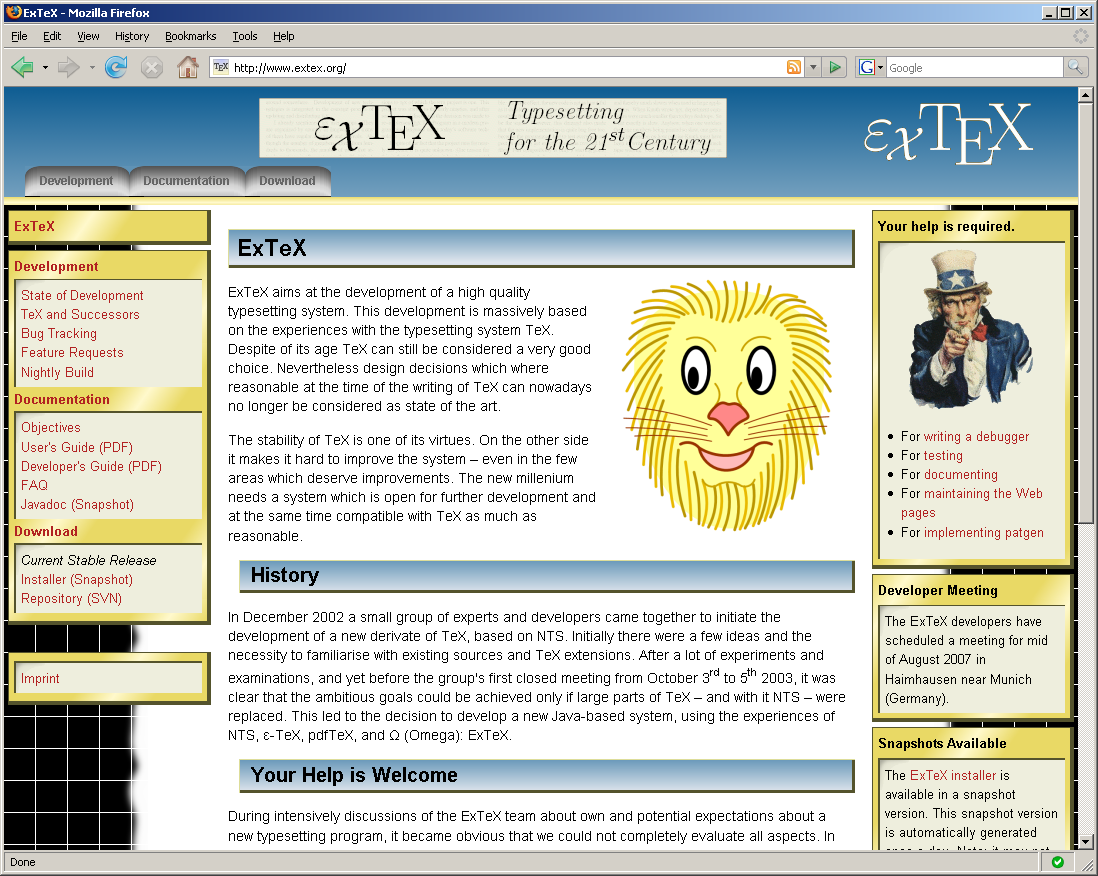
\includegraphics[width=.5\textwidth]{img/www-extex-org}
  \caption{\texttt{www.extex.org}}
  \label{fig:www.exetex.org}
\end{figure}
There is a web site devoted to \ExTeX.\index{WWW}\index{Web Site} This
web site (see figure~\ref{fig:www.exetex.org}) can be reached via the
URL\index{www.extex.org}
\begin{quotation}
  \url{http://www.extex.org}
\end{quotation}


\section{Mailing Lists}
%@author Gerd Neugebauer

If you are ready to try \ExBib{} you might as well want to join a
mailing list to get in contact with the community.\index{mailing list}

\begin{quotation}
  \url{http://www.dante.de/listman/extex}
\end{quotation}


\section{Reporting Bugs}
%@author Gerd Neugebauer


If you find any bugs in \ExBib\ you can submit them 
%either 
via a HTML form.
% or via email. 
You can find the HTML form at
\begin{quotation}
  \url{http://www.extex.org/bugs}
\end{quotation}
%Emails containing the description can be sent to
%\begin{quotation}
%  \href{mailto:extex-bugs@dante.de}{extex-bugs@dante.de}
%\end{quotation}

Please include in your description 
\begin{itemize}
\item the source of a \emph{minimal} example showing the problem
\item the log file resulting from running this example
\item a description why you think that something went wrong and what
  the expected result would be
\item a description of the environment you are using (host
  architecture, operating system, Java version)
\end{itemize}

\endinput
%
% Local Variables: 
% mode: latex
% TeX-master: "exbib-users"
% End: 

%%*****************************************************************************
%% $Id: started.tex,v 0.00 2008/05/01 17:52:50 gene Exp $
%%*****************************************************************************
%% Author: Gerd Neugebauer
%%-----------------------------------------------------------------------------

\chapter{Getting Started}
%@author Gerd Neugebauer

In this chapter we describe the steps you can take to get \ExBib\ up
and running. We try to use as few as possible premises. Thus it should
be not too hard to get started.

\section{Prerequisites}
%@author Gerd Neugebauer

\subsection{Java}
%@author Gerd Neugebauer

You need to have Java 5\index{Java} or later installed on your
system. You can get Java for a several systems directly from
\url{java.sun.com}. Download and install it according to the
installation instructions for your environment.

To check that you have an appropriate Java on your path you can use
the command \texttt{java} with the argument \texttt{-version}. This
can be seen in the following example:

\lstset{morecomment=[l]{\#}}%
\begin{lstlisting}{morecomment=[l][keywordstyle]{>}}
# java -version
java version "1.5.0_04"
Java(TM) 2 Runtime Environment, Standard Edition (build 1.5.0_04-b05)
Java HotSpot(TM) Client VM (build 1.5.0_04-b05, mixed mode)
#
\end{lstlisting}


\subsection{TEXMF}
%@author Gerd Neugebauer

If you want to use more than the pure \ExBib\ engine, styles can be
inherited from a texmf tree\index{texmf}. \ExBib\ itself does not
contain a full texmf tree. It comes just with some rudimentary files
necessary for testing and getting started. Thus you should have
installed a texmf tree, e.g. from a \TeX Live\index{TeXlive@\TeX Live}
installation. This can be found on the
\href{http://www.ctan.org}{Comprehensive \TeX\ Archive Network
  (CTAN)}\index{CTAN}.

There is no need to install the texmf tree in a special place. You
have to tell \ExBib\ anyhow where it can be found. It is even possible
to work with several texmf trees.

One requirement for the texmf trees is that they have a file database
(\File{ls-R}). \ExBib\ can be configured to work without it, but then
\ExBib\ is deadly slow. Thus you do not really want to try this
alternative.


\section{Getting \ExBib}
%@author Gerd Neugebauer

\subsection{Getting the Installer}
%@author Gerd Neugebauer

The simplest way to get \ExBib\ up and running is to use the \ExBib\ 
installer. This installer\index{installer} is distributed as one file
\File{ExBib-setup.jar}. You can download it from

\begin{quotation}
  \url{http://www.extex.org/download/}
\end{quotation}

If you have got the installer there is no need for you to get the
sources as well. Nevertheless the soruces can be retrieved via
Subversion from
\begin{quotation}
  \url{https://svn.berlios.de/svnroot/repos/extex/trunk/ExBib}
\end{quotation}


\section{Installing \ExBib}\label{sec:install}
%@author Gerd Neugebauer

The installation of \ExBib\ works with the \ExBib\ installer. This
installer is named \File{ExBib-setup.jar}. You can start the installer
with the following command line:\index{installer}

\begin{lstlisting}{}
# java -jar ExTeX-setup.jar
\end{lstlisting}

On Windows\index{Windows} with a properly installed Java\index{Java}
you can also start the installer by double-clicking
\texttt{ExBib-setup.jar} in the Explorer\index{Explorer}. This might
work on other windowing systems as well.

\begin{figure}[!ht]
  \centering
  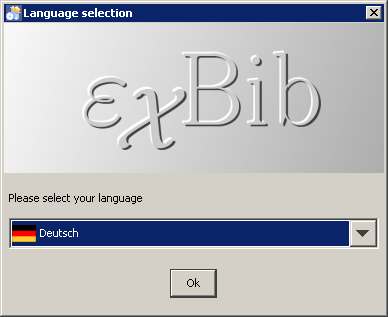
\includegraphics[width=.45\textwidth]{img/inst1}\hfill
  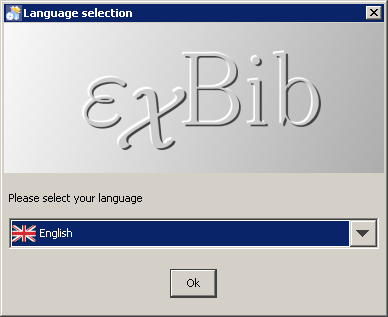
\includegraphics[width=.45\textwidth]{img/inst2}
  \caption{The Language Selection in the Installer}
  \label{fig:inst1}
\end{figure}
The installer provides a graphical user interface with a wizard
guiding you through the installation process. The first dialog is
shown in figure~\ref{fig:inst1}. As you can see you can select one of
several languages for the installation process. This selection just
effects the language used to communicate during the instanllation
process.  Currently the languages English and German are supported.
There might be some more at the time you are performing the
installation.\index{installer!language}\index{language!installer}

Note that the language selection covers the installer only. \ExBib\ 
can be run under different language environments as well. This is
controlled by a setting at run-time. Currently only an English and
a German language binding for \ExBib\ are provided.\index{language}

\begin{figure}[!ht]
  \centering
  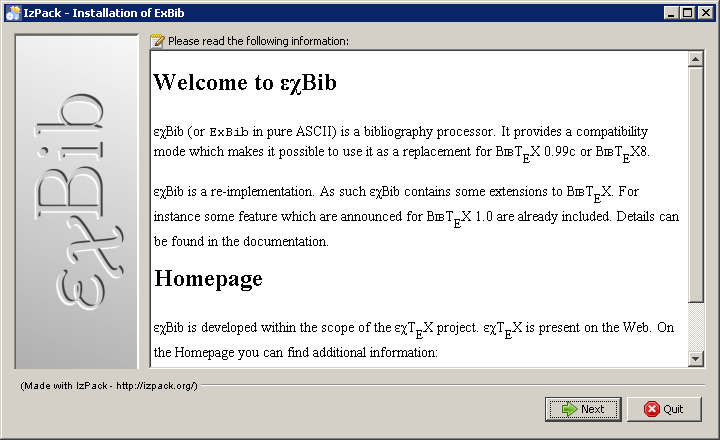
\includegraphics[width=.45\textwidth]{img/inst3}
  \caption{Welcome to \ExBib}
  \label{fig:inst2}
\end{figure}

The next panel shows a welcome message showing what this installer is
about (see figure~\ref{fig:inst2}). Since you are reading this
document there is nothing new for you.

\begin{figure}[!ht]
  \centering
  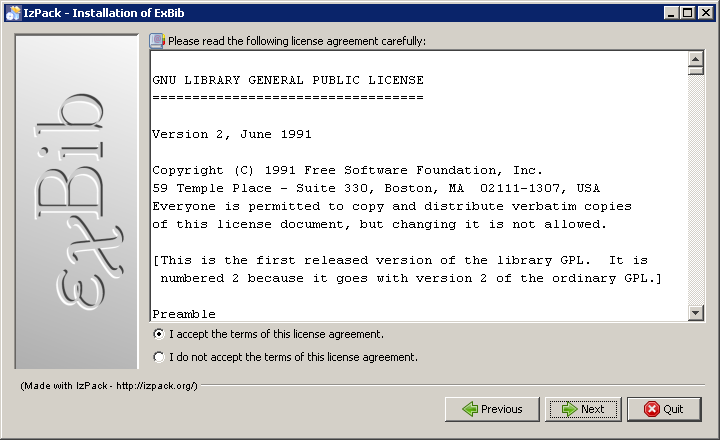
\includegraphics[width=.45\textwidth]{img/inst4}
  \caption{Accepting the Licence}
  \label{fig:inst3}
\end{figure}

Now the license of \ExBib\ is presented (see figure~\ref{fig:inst3}).
It is there to remind you that there is something like a license. You
can not do everything with the software. But the limitations are very
minimalistic. Usually it should not really affect you -- especially
when you are migrating from \BibTeX.

Note that the license is the LGPL. In contrast to the GPL it does not
infect other software build from \ExBib\ or containing it.

\begin{figure}[!ht]
  \centering
  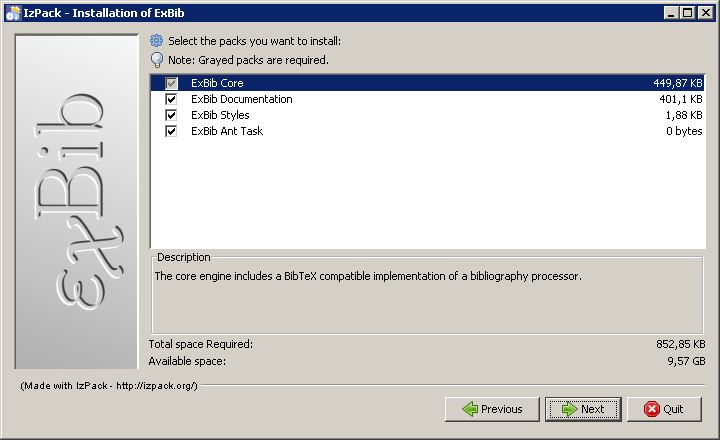
\includegraphics[width=.45\textwidth]{img/inst5}
  \caption{Selecting the Packages}
  \label{fig:inst4}
\end{figure}

Next the packages to be installed can be selected (see
figure~\ref{fig:inst4}). The core packages is needed in any case. Thus
it can not be deselected. The other packages can be freely choosen
from.

Whenever you select a package in the list a short discription of the
package is displayed.

\begin{figure}[!ht]
  \centering
  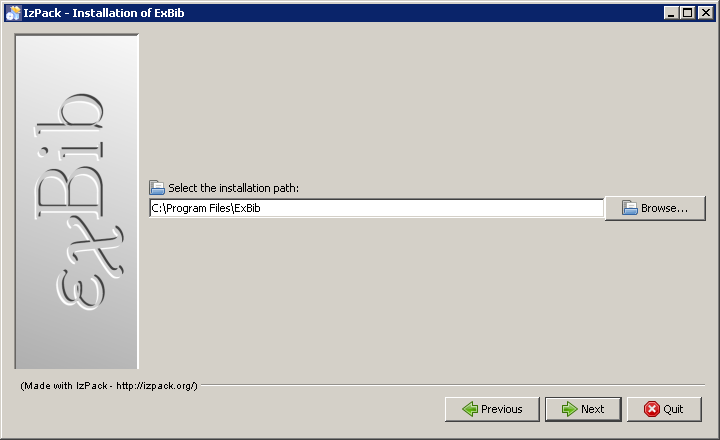
\includegraphics[width=.45\textwidth]{img/inst6}
  \caption{Selecting the Installation Directory}
  \label{fig:inst5}
\end{figure}

Finally the installation directory has to be selected (see
figure~\ref{fig:inst5}). The installation directory (see also
section~\ref{sec:inst.dir}) is the only directory the \ExBib\ 
installer creates files in. Usually is should be separate from other
directories. For instance the value \verb|C:\Program Files\ExBib| on
Windows or \verb|/opt/ExBib| on Unix are sensible values. Nevertheless
the installation can also be performed in your home directory if you
do not have writing permissions in the global directories.

This is the last decision you have to make.

\begin{figure}[!ht]
  \centering
  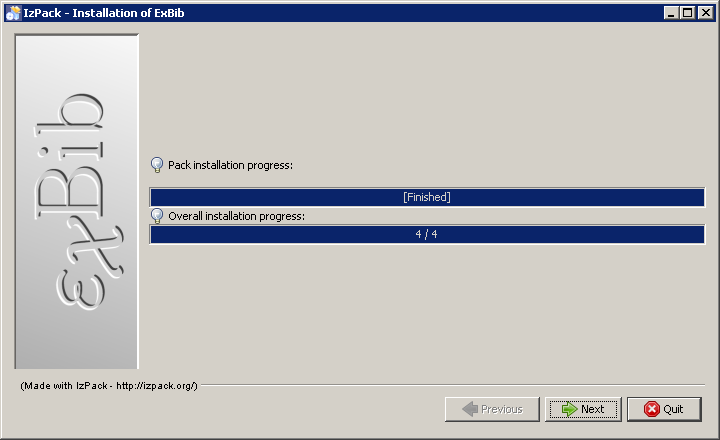
\includegraphics[width=.45\textwidth]{img/inst7}
  \caption{Progress of the Installation}
  \label{fig:inst6}
\end{figure}

Now the installation is performed. A progress panel is shown during
the installation (see figure~\ref{fig:inst6}). As a result the
installation directory is created and filled (see also
section~\ref{sec:inst.dir})

\begin{figure}[!ht]
  \centering
  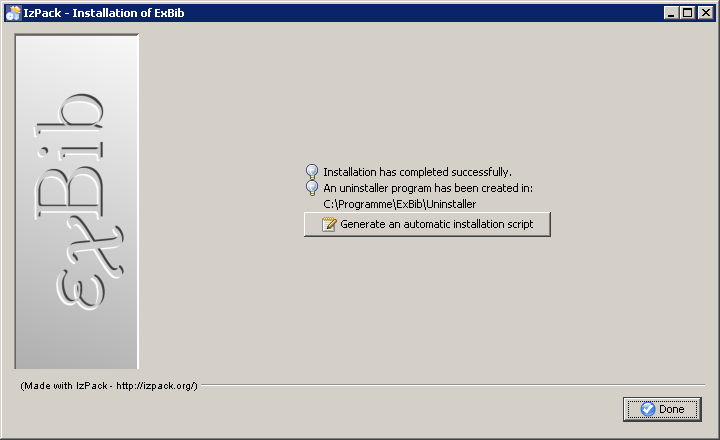
\includegraphics[width=.45\textwidth]{img/inst8}
  \caption{Saving the Installation Settings}
  \label{fig:inst7}
\end{figure}

When the installation is completed you get the chance to save the
settings for unattended replay (see figure~\ref{fig:inst7}). See
section~\ref{sec:replay} for details.


Finally you have to make sure that the executables \Prog{exbib} or
\Prog{exbib.bat} are on your path for executables.\index{path} This
can be achieved by modifying the environment variable \verb|PATH| in a
Unix environment or setting \verb|path| in the system settings on
Windows.


\subsection{The Installation Directory}\label{sec:inst.dir}
%@author Gerd Neugebauer

During the installation you choose a directory where \ExBib\ lives.
This is called the installation directory. An example of the contents of the
installation directory can be seen in figure~\ref{fig:inst.dir}.

\begin{figure}[!ht]
  \centering
\begin{DirList}{200pt}{250pt}
  \TOPDIR(0,30){ExBib}
  \DIR(3,28)2{Uninstaller}
  \FILE(6,26)2{uninstaller.jar}
  \DIR(3,24){4.75}{bin}
  \FILE(6,22)2{exbib}
  \FILE(6,20){2.5}{exbib.bat}
  \FILE(6,18){2.5}{exbibutil}
  \FILE(6,16){2.5}{exbibutil.bat}
  \DIR(3,14){10.75}{doc}
  \FILE(6,12)2{exbib-manual.pdf}
  \DIR(3,10){4.75}{lib}
  \FILE(6,8){2}{ExBib-core.jar}
  \FILE(6,6){2.5}{ExBib-Main.jar}
  \FILE(6,4){2.5}{ExBib-styles.jar}
  \FILE(6,2){2.5}{ExTeX-resource.jar}
  \FILE(3,0){10.75}{LICENSE.txt}
\end{DirList}
  \caption{The Installation Directory}

  \label{fig:inst.dir}
\end{figure}

The directory \File{Uninstaller} contains the uninstaller. It can be
used to get rid of \ExBib\ -- even when I don't know why you should
want to. For details see section~\ref{sec:uninst}

The directory \File{bin} contains the binaries. This directory should
be put onto the path for executables. Note that currently all
executables are installed on any platform. On Windows the programs
without extension can be useful within the cygwin world. On Unix the
files with the extension \verb|.bat| can be simply ignored.

The directory \File{doc} contains documentation if the documentation
package has been selected during the installation.

The directory \File{lib} contains the libraries used by \ExBib.


\subsection{Replaying an Installation}\label{sec:replay}
%@author Gerd Neugebauer

Sometimes it is desirable to perform an installation on several
similar machines. This means that the answers to the questions in the
installer are the same. This process can be automated.

In figure~\ref{fig:inst7} you can see the last screen of the
installer. Here you have the possibility to select the button
``Generate an automatic installation script''. This produces an XML
file which can be passed to the installer to avoid the
dialogs.\index{installer}\index{installation script}

Suppose you have named the file \texttt{replay.xml} in the file
selector which pops up when the button has been pressed. Then you can
replay the installation with the following command invocation:

\begin{lstlisting}{}
# java -jar ExBib-setup.jar replay.xml
\end{lstlisting}

This supposes that the two files \File{ExTeX-setup.jar} and
\texttt{replay.xml} are in the current directory.

\subsection{Uninstalling \ExBib}\label{sec:uninst}
%@author Gerd Neugebauer

The files installed by the installer (see section~\ref{sec:install})
can be removed from the system. For this purpose an uninstaller is
provided in the subdirectory \File{Uninstaller} of the \ExBib\
installation directory. It is named \File{uninstaller.jar}. It can be
invoked by double clicking or invoking it on the command line as follows:

\begin{lstlisting}{}
# java -jar uninstaller.jar
\end{lstlisting}

\begin{figure}[!h]
  \centering
  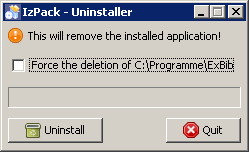
\includegraphics[width=.45\textwidth]{img/uninst1}
  \caption{Confirming the Uninstallation}
  \label{fig:uninst1}
\end{figure}

When the uninstaller starts it asks for configmation (see
figure~\ref{fig:uninst1}). Nothing is changed before the confirmation
is given.

\begin{figure}[!h]
  \centering
  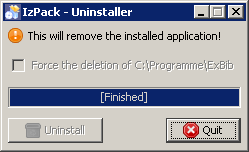
\includegraphics[width=.45\textwidth]{img/uninst2}
  \caption{The Uninstaller Finished}
  \label{fig:uninst2}
\end{figure}

The uninstaller shows a progress bar (see figure~\ref{fig:uninst2}).
When the uninstaller has finished its work all files and directories
installed with the installer have been removed. Modified and other
files are left untouched.

You can uninstall \ExBib\ by simply removing the installation
directory. But this is unsave since all local modification are lost as
well.

%%*****************************************************************************
%% $Id: cli-exbib.tex,v 0.00 2008/05/02 17:03:28 gene Exp $
%%*****************************************************************************
%% Author: Gerd Neugebauer
%%-----------------------------------------------------------------------------


%------------------------------------------------------------------------------
\section{Running \ExBib}
%@author Gerd Neugebauer

Currently \ExBib\ can be run from the command line. In this respect it
is more or less identical to \BibTeX\ and can be used as a plug-in
replacement. In addition the features of \BibTeX~8 are present as
well. The marks in the margin indicate where the different features
are coming from.

%-----------------------------------------
%
%The following sample show a simple invocation of \ExBib\ without any
%command line arguments.
%
%{\lstset{morecomment=[l]{*}}%
%\begin{lstlisting}{}
%# exbib
%This is exbib, Version 0.0 (TeX compatibility mode)
%**\relax
%
%*\end
%
%No pages of output.
%Transcript written on ./texput.log.
%\end{lstlisting}}
%
%In this case \ExTeX\ enters interaction with the user and asks for an
%input file. This is indicated by the two asterisks. We have entered
%\macro{relax} here to indicate that we are not willing to pass in a
%file name. The \ExTeX\ system asks us to enter some command --
%indicted by the single asterisk. Here we have entered \macro{end} to
%indicate that we want to finish the processing. Thus \ExTeX\ 
%terminates normally.
%
%\INCOMPLETE
%
%{\lstset{morecomment=[l]{*}}%
%\begin{lstlisting}{}
%# extex plain
%This is ExTeX, Version 0.0 (TeX compatibility mode)
%(plain Preloading the plain format: codes, registers, parameters, fonts,
%more fonts, macros, math definitions, output routines, hyphenation(hyphen))
%*\dump
%Beginning to dump on file plain.fmt
%
%*\end
%
%No pages of output.
%Transcript written on ./plain.log.
%\end{lstlisting}}
%
%
%--------------------------------
%The invocation of the executable \Prog{extex} can be controlled by
%large number of command line arguments. Those command line arguments
%are described in the following list:
%
%\begin{description}
%\item[\Arg{code}]\ \\
%  This parameter contains \ExTeX\ code to be executed directly. The
%  execution is performed after any code specified in an input file. On
%  the command line the code has to start with a backslash. This
%  restriction does not hold for the property settings.
%
%  This command line argument sets the property \Property{extex.code}
%  
%\item[\Arg{file}]\ \\
%  This parameter contains the file to read from. A file name may not
%  start with a backslash or an ambercent. It has no default.
%
%  This command line argument sets the property \Property{extex.file}.
%  
%\item[\CLI{-} \Arg{file}]\ \\
%  This parameter terminates the normal processing of arguments. The
%  next argument -- if present -- is interpreted as input file. With
%  this construction it is possible to process an input file which
%  starts with one of the special characters \verb|\| or \verb|&|.
%
%  This command line argument sets the property \Property{extex.file}
%  if a file argument is present.
%
%\item[\CLI{configuration} \Arg{resource}]\ \\
%  This parameter contains the name of the configuration resource to
%  use. This configuration resource is sought on the class path.
%  
%  This command line argument sets the property \Property{extex.config}.
%  
%\item[\CLI{copyright}]\ \\
%  This command line option produces a copyright notice on the standard
%  output stream and terminates the program afterwards.
%
%\item[\tt\&\Arg{format}]\index{\&}
%\item[\CLI{fmt} \Arg{format}]\ \\
%  This parameter contains the name of the format to read. An empty
%  string denotes that no format should be read. This is the default.
%
%  This command line argument sets the property \Property{extex.format}.
%  
%\item[\CLI{debug} \Arg{spec}]\ \\
%  This command line parameter can be used to instruct the program to
%  produce debugging output of several kinds. The debug output is
%  written to the log file. The specification \Arg{spec} is interpreted
%  left to right. Each character is interpreted according to the
%  following table:
%
%  \begin{tabular}{lp{.4\textwidth}l}\toprule
%    \textit{Spec}& \textit{Description}& \textit{See} \\\midrule
%    F& 	This specifier contains the indicator whether or not to trace
%    the searching for input files. & 	\Property{extex.trace.input.files}\\
%    f& 	This specifier contains the indicator whether or not to trace
%    the searching for font files.&      \Property{extex.trace.font.files}\\
%    M& 	This specifier contains the indicator whether or not to trace
%    the execution of macros.&	 	\Property{extex.trace.macros}\\
%    T& 	This specifier contains the indicator whether or not to trace
%    the work of the tokenizer.& 	\Property{extex.trace.tokenizer}\\
%    \bottomrule
%  \end{tabular}
%
%  The following example shows a possible invocation with this
%  parameter: 
%\begin{lstlisting}{}
%# extex -debug FfMT abc.tex
%This is ExTeX, Version 0.0 (TeX compatibility mode)
%...
%\end{lstlisting}
%  
%\item[\CLI{halt-on-error}]\ \\
%  This parameter contains the indicator whether the processing should
%  halt after the first error which has been encountered.
%
%  This command line argument sets the property \Property{extex.halt.on.error}.
%  
%\item[\CLI{help}]\ \\
%  This command line option produces a short usage description on the
%  standard output stream and terminates the program afterwards.
%  
%\item[\CLI{ini}]\ \\
%  If set to true then act as ini\TeX.\index{initex@ini\TeX} In this
%  case no format has to be preloaded. All parameters are set to the
%  "`factory settings"'.
%
%  This command line argument sets the property \Property{extex.ini}.
%
%  The following example shows a possible invocation with this
%  parameter: 
%\begin{lstlisting}{}
%# extex -ini abc.tex
%This is ExTeX, Version 0.0 (TeX compatibility mode)
%...
%\end{lstlisting}
%  
%\item[\CLI{interaction} \Arg{mode}]\ \\
%  This parameter contains the interaction mode. possible values are
%  the numbers 0\dots3 and the symbolic names \Mode{batchmode} (0),
%  \Mode{nonstopmode} (1), \Mode{scrollmode} (2), and
%  \Mode{errorstopmode} (3).
%
%  This command line argument sets the property \Property{extex.interaction}.
%  
%  The following example shows a possible invocation with this
%  parameter:
%\begin{lstlisting}{}
%# extex -interaction batchmode abc.tex
%This is ExTeX, Version 0.0 (TeX compatibility mode)
%...
%\end{lstlisting}
%
%\item[\CLI{job-name} \Arg{name}]\ \\
%  This parameter contains the name of the job. It is overwritten if a
%  file is given to read from. In this case the base name of the input
%  file is used instead.
%
%  This command line argument sets the property \Property{extex.jobname}.
%  
%\item[\CLI{language} \Arg{language}]\ \\
%  This parameter contains the name of the locale to be used for the
%  messages.
%
%  This command line argument sets the property \Property{extex.lang}.
%  
%\item[\CLI{output} \Arg{format}]\ \\
%  This parameter contains the output format. This logical name is
%  resolved via the configuration.
%
%  This command line argument sets the property \Property{extex.output}.
%
%  The following example shows a possible invocation with this
%  parameter: 
%\begin{lstlisting}{}
%# extex -output pdf abc.tex
%This is ExTeX, Version 0.0 (TeX compatibility mode)
%\end{lstlisting}
%  
%\item[\CLI{progname} \Arg{name}]\ \\
%  This parameter can be used to overrule the name of the program shown
%  in the banner and the version information.  The following example
%  shows a possible invocation and the resulting output:
%
%\begin{lstlisting}{}
%# extex -progname XeTxE -version
%This is XeTxE, Version 0.0 (1.4.2_06)
%#
%\end{lstlisting}
%
%  This command line argument sets the property \Property{extex.progname}.
%  
%\item[\CLI{texinputs} \Arg{path}]\ \\
%  This parameter contains the additional directories for searching
%  \ExTeX\ input files.  The directories are separated by the
%  system-dependant separator.  This separator is a colon (\verb|:|) on
%  Unix\index{Unix} and the semicolon (\verb|;|) on
%  Windows\index{Windows}.
%  
%  This command line argument sets the property
%  \Property{extex.texinputs}.
%  
%\item[\CLI{texmfoutputs} \Arg{dir}]\ \\
%  This parameter contains the name of the property for the fallback if
%  the output directory fails to be writable.
%  
%  This command line argument sets the property
%  \Property{extex.outputdir.fallback}.
%  
%\item[\CLI{texoutputs} \Arg{dir}]\ \\
%  This parameter contain the directory where output files should be
%  created.
%
%  This command line argument sets the property \Property{extex.outputdir}.
%  
%\end{description}
%

\subsection{Command Line Parameters}
%@author Gerd Neugebauer

\subsubsection{The Aux File}

\begin{description}
\item[\Arg{file}]\ \\
  This parameter contains the aux file to read from. A file name may not
  start with minus sign. It has no default.
  \begin{lstlisting}{}
    # extex doc.aux
    This is exbib, Version 0.1
  \end{lstlisting}
  
\item[\CLI{} \Arg{file}]
\item[\CLI{-} \Arg{file}]\ \\
  This parameter terminates the intercepts processing of arguments. The
  next argument -- if present -- is interpreted as input file. With
  this construction it is possible to process an input file which
  starts with the special character \verb|-|.
  \begin{lstlisting}{}
    # extex -- doc.aux
    This is exbib, Version 0.1
  \end{lstlisting}

\end{description}

The file name given is used to determine the name of an aux file. This
means that it is either the name of an aux file or the base name which
is augmented by the extension \texttt{.aux} to find the aux file.

The main control information is taken from this aux file. This means
it contains the foloowing items:

\begin{itemize}
\item The database files to consult.
\item The citations to extract.
\item The bst to use for formatting.
\item References to other aux files to consult as well.
\end{itemize}

\subsubsection{Version Information and Help}

\begin{description}
\item[\CLI{-copying}]\ \\
  This command line option produces a copyright notice on the standard
  output stream and terminates the program afterwards.
  \begin{lstlisting}{}
# exbib --copying
                 GNU LESSER GENERAL PUBLIC LICENSE
                      Version 2.1, February 1999
Copyright (C) 1991, 1999 Free Software Foundation, Inc.
    59 Temple Place, Suite 330, Boston, MA  02111-1307  USA
Everyone is permitted to copy and distribute verbatim copies
of this license document, but changing it is not allowed.
[This is the first released version of the Lesser GPL.  It also counts
as the successor of the GNU Library Public License, version 2, hence
the version number 2.1.]
                           Preamble
 The licenses for most software are designed to take away your
freedom to share and change it.  By contrast, the GNU General Public
Licenses are intended to guarantee your freedom to share and change
free software--to make sure the software is free for all its users.
    ...
  \end{lstlisting}

\item[\CLI{h}]
\item[\CLI{?}]
\item[\CLI{-help}]\ \\
  This command line option produces a short usage description on the
  standard output stream and terminates the program afterwards.
  \begin{lstlisting}{}
# exbib --help
This is exbib, Version 0.1
Usage: exbib <options> file
The following options are supported:
        -[-] <file>
                Use this argument as file name -- even when it looks like an option.
        --trad[itional] | -7
                operate in the original 7-bit mode.
        --8[bit] | -8
                force 8-bit mode, no CS file used.
    ...
\end{lstlisting}
  
\item[\CLI{-release}]\ \\
  This command prints the release number to stdout and exits the
  program. This can be used to enable external programs to easily
  determine the version number of \ExBib.
\begin{lstlisting}{}
# exbib --release
0.1
#
\end{lstlisting}

\item[\CLI{-version}]\ \\
  This command line parameter forces that the version information is
  written to standard output and the program is
  terminated.\index{version} The version of \ExBib\ is shown. The
  following example shows a possible invocation and the resulting
  output:
\begin{lstlisting}{}
# exbib --version
This is exbib, Version 0.1
Copyright (C) 2002-2008 Gerd Neugebauer (mailto:gene@gerd-neugebauer.de).
There is NO warranty.  Redistribution of this software is
covered by the terms of the GNU Library General Public License.
For more information about these matters, use the command line
switch -copying.
#
\end{lstlisting}
\end{description}


\subsubsection{Internationalization}

\begin{description}
\item[\CLI{L} \Arg{lang}]
\item[\CLI{-language} \Arg{lang}]\ \\
  This command line option switches the language to the given
  language. The argument is a two-letter ISO code for a language. For
  instance the value \texttt{en} represents English and \texttt{de}
  represents German.

  The language is used to select the appropriate messages for logging
  and error messages. If the given language is not supported English
  is silently used as fallback.
\begin{lstlisting}{}
# exbib --language de --help
Dies ist exbib, Version 0.1
Copyright (C) 2002-2008 Gerd Neugebauer (mailto:gene@gerd-neugebauer.de).
There is NO warranty.  Redistribution of this software is
covered by the terms of the GNU Library General Public License.
For more information about these matters, use the command line
switch -copying.
#
\end{lstlisting}
\end{description}


\subsubsection{Configurations}

\ExBib\ is highly configurable. The whole system is assembled from
components at run time. The assembly is controlled from a set of
configuration files. There is one central configuration file which
acts as entry point.

\begin{description}
\item[\CLI{c} \Arg{config}]
\item[\CLI{-configuration} \Arg{config}]\ \\
  Set the configuration file to be used for assenbling \ExBib. The
  default is the configuration \texttt{exbib}.
\begin{lstlisting}{}
# exbib --configuration bibtex099 doc.aux
This is exbib, Version 0.1
...
\end{lstlisting}

\item[\CLI{-bibtex}]
\item[\CLI{-strict}]\ \\
  Use the configuration \texttt{bibtex099} for assembling \ExBib.
\begin{lstlisting}{}
# exbib --bibtex doc.aux
This is exbib, Version 0.1
...
\end{lstlisting}
\end{description}

The following configurations are present in the distribution.

\begin{description}
\item[exbib]\ \\
  This is the default configuration which includes all features
  described in this reference manual.
\item[bibtex099]\ \\
  This is the configuration for backward compatibility. It emulates
  the features of \BibTeX~0.99c as closely as possible. The extended
  features of \ExBib\ are not present in this configuration.
\end{description}

\subsubsection{Encodings}

The internal representation of characters uses Unicode. In general it
is necessary to translate from and to the internal representation when
reading and writing files. For this purpose the encodings to be used
can be configured.

The default is to use the default encoding for the platform \ExBib\ is
currently running. Thus it is not necessary to specify an encoding at
all.

It is guaranteed that at least the following encodings are present on
your system:

\begin{description}
\item[US-ASCII] 
  Seven-bit ASCII.
\item[ISO-8859-1] 
  ISO Latin Alphabet 1
\item[UTF-8] 
  Eight-bit UCS Transformation Format.
\item[UTF-16BE] 
  Sixteen-bit UCS Transformation Format in big-endian byte order.
\item[UTF-16LE] 
  Sixteen-bit UCS Transformation Format in little-endian byte order.
\item[UTF] Sixteen-bit UCS Transformation Format; the byte order
  identified by an optional byte-order mark.
\end{description}

The following list has been obtained at the time of writing this
document (on a Windows system):

\noindent
\begin{multicols}5\obeylines\scriptsize\parindent=0pt
  Big5
  Big5-HKSCS
  EUC-JP
  EUC-KR
  GB18030
  GB2312
  GBK
  IBM-Thai
  IBM00858
  IBM01140
  IBM01141
  IBM01142
  IBM01143
  IBM01144
  IBM01145
  IBM01146
  IBM01147
  IBM01148
  IBM01149
  IBM037
  IBM1026
  IBM1047
  IBM273
  IBM277
  IBM278
  IBM280
  IBM284
  IBM285
  IBM297
  IBM420
  IBM424
  IBM437
  IBM500
  IBM775
  IBM850
  IBM852
  IBM855
  IBM857
  IBM860
  IBM861
  IBM862
  IBM863
  IBM864
  IBM865
  IBM866
  IBM868
  IBM869
  IBM870
  IBM871
  IBM918
  ISO-2022-CN
  ISO-2022-JP
  ISO-2022-JP-2
  ISO-2022-KR
  ISO-8859-1
  ISO-8859-13
  ISO-8859-15
  ISO-8859-2
  ISO-8859-3
  ISO-8859-4
  ISO-8859-5
  ISO-8859-6
  ISO-8859-7
  ISO-8859-8
  ISO-8859-9
  JIS\_X0201
  JIS\_X0212-1990
  KOI8-R
  KOI8-U
  Shift\_JIS
  TIS-620
  US-ASCII
  UTF-16
  UTF-16BE
  UTF-16LE
  UTF-32
  UTF-32BE
  UTF-32LE
  UTF-8
  windows-1250
  windows-1251
  windows-1252
  windows-1253
  windows-1254
  windows-1255
  windows-1256
  windows-1257
  windows-1258
  windows-31j
  x-Big5-Solaris
  x-euc-jp-linux
  x-EUC-TW
  x-eucJP-Open
  x-IBM1006
  x-IBM1025
  x-IBM1046
  x-IBM1097
  x-IBM1098
  x-IBM1112
  x-IBM1122
  x-IBM1123
  x-IBM1124
  x-IBM1381
  x-IBM1383
  x-IBM33722
  x-IBM737
  x-IBM834
  x-IBM856
  x-IBM874
  x-IBM875
  x-IBM921
  x-IBM922
  x-IBM930
  x-IBM933
  x-IBM935
  x-IBM937
  x-IBM939
  x-IBM942
  x-IBM942C
  x-IBM943
  x-IBM943C
  x-IBM948
  x-IBM949
  x-IBM949C
  x-IBM950
  x-IBM964
  x-IBM970
  x-ISCII91
  x-ISO-2022-CN-CNS
  x-ISO-2022-CN-GB
  x-iso-8859-11
  x-JIS0208
  x-JISAutoDetect
  x-Johab
  x-MacArabic
  x-MacCentralEurope
  x-MacCroatian
  x-MacCyrillic
  x-MacDingbat
  x-MacGreek
  x-MacHebrew
  x-MacIceland
  x-MacRoman
  x-MacRomania
  x-MacSymbol
  x-MacThai
  x-MacTurkish
  x-MacUkraine
  x-MS950-HKSCS
  x-mswin-936
  x-PCK
  x-UTF-16LE-BOM
  X-UTF-32BE-BOM
  X-UTF-32LE-BOM
  x-windows-50220
  x-windows-50221
  x-windows-874
  x-windows-949
  x-windows-950
  x-windows-iso2022jp
\end{multicols}

The following command line options are related to encodings:

\begin{description}
\item[\CLI{-availableCharsets}]\ \\
  This instruction lists the available character sets on standard
  output and exits the program.
\begin{lstlisting}{}
# exbib --availableCharsets
Big5
Big5-HKSCS
EUC-JP
EUC-KR
GB18030
GB2312
GBK
IBM-Thai
IBM00858
IBM01140
...
\end{lstlisting}

\item[\CLI{E} \Arg{enc}]
\item[\CLI{-bib-encoding} \Arg{enc}]
\item[\CLI{-bib.encoding} \Arg{enc}]\ \\
  Set the configuration for reading bib database files. The encoding
  needs to be a valid character set.
\begin{lstlisting}{}
# exbib --bib-encoding=UTF8 doc.aux
...
\end{lstlisting}

\item[\CLI{e} \Arg{enc}]
\item[\CLI{-encoding} \Arg{enc}]\ \\

  \INCOMPLETE
\begin{lstlisting}{}
# exbib --encoding=UTF8 doc.aux
...
\end{lstlisting}

\end{description}
%        --e[ncoding] | -e <enc>
%        	Nutze das gegebene Encoding f�r die Ausgabedatei.

\subsubsection{CS Files}

\begin{description}
\item[\CLI{-csfile} \Arg{csfile}]\ \\

  \INCOMPLETE
\begin{lstlisting}{}
# exbib --csfile=iso8859-7.csf doc.aux
...
\end{lstlisting}
%        --cs[file] <csfile>
%        	Nutze das csf zur Definition von Zeichen und Sortierung.

\item[\CLI{7}]
\item[\CLI{-traditional}]\ \\
  \INCOMPLETE
\begin{lstlisting}{}
# exbib --traditional doc.aux
...
\end{lstlisting}
%        --trad[itional] | -7
%        	arbeite im originalen 7-Bit-Modus.

\item[\CLI{8}]
\item[\CLI{-8bit}]\ \\
  \INCOMPLETE
\begin{lstlisting}{}
# exbib --8bit doc.aux
...
\end{lstlisting}
%        --8[bit] | -8
%        	Erzwinge  8-Bit-Modus, es wird keine CS-Datei eingesetzt.
\end{description}

\subsubsection{Redirecting Output}

\begin{description}
\item[\CLI{l} \Arg{file}]
\item[\CLI{-logfile} \Arg{file}]\ \\
  This option redirects the log output to the given file. The default
  name of the log file is derived from the base name of the aux file
  by appending \texttt{.blg}. This option overwrites this default.
  behaviour.
\begin{lstlisting}{}
# exbib --logfile=my.log doc.aux
...
\end{lstlisting}

  If the given file name is the value \texttt{-} then the output is
  sent to stdout.
\begin{lstlisting}{}
# exbib --logfile=- doc.aux
...
\end{lstlisting}

  If the given file name is empty then the log output is discarted.
\begin{lstlisting}{}
# exbib --logfile= doc.aux
...
\end{lstlisting}

\item[\CLI{o} \Arg{file}]
\item[\CLI{-output} \Arg{file}]
\item[\CLI{-outfile} \Arg{file}]\ \\
  This option redirects the output to the given file. The default
  name of the output file is derived from the base name of the aux file
  by appending \texttt{.bbl}. This option overwrites this default.
  behaviour.
\begin{lstlisting}{}
# exbib --outfile=my.out doc.aux
...
\end{lstlisting}

  If the given file name is the value \texttt{-} then the output is
  sent to stdout.
\begin{lstlisting}{}
# exbib --outfile=- doc.aux
...
\end{lstlisting}

  If the given file name is empty then the output is discarted.
\begin{lstlisting}{}
# exbib --outfile= doc.aux
...
\end{lstlisting}

\end{description}


\subsubsection{Changing the Style}

\begin{description}
\item[\CLI{b} \Arg{style}]
\item[\CLI{-bst} \Arg{style}]\ \\
  This option sets the name of the bib style to be used. The bib style
  is normally read from the aux file. This instruction overrules
  whatever the aux file contains.
\begin{lstlisting}{}
# exbib --bst=alpha doc.aux
...
\end{lstlisting}

\end{description}

\subsubsection{min crossrefs}

\begin{description}
\item[\CLI{M} \Arg{n}]
\item[\CLI{-min-crossrefs} \Arg{n}]
\item[\CLI{-min.crossrefs} \Arg{n}]
\item[\CLI{-min\_crossrefs} \Arg{n}]\ \\
  This option sets the minimum number of crossreferences before an
  entry is not collaped.
\begin{lstlisting}{}
# exbib --min-crossrefs=4 doc.aux
...
\end{lstlisting}

\end{description}

\subsubsection{Naming the Program}

\begin{description}
\item[\CLI{p} \Arg{name}]
\item[\CLI{-progname} \Arg{name}]
\item[\CLI{-program-name} \Arg{name}]
\item[\CLI{-program.name} \Arg{name}]\ \\
  This option sets the name of the porogram. Thus it is possible to
  influence how the program calls itself in logging and error messages
  from outside .
\begin{lstlisting}{}
# exbib --progname=BibTeX doc.aux
This is BibTeX, Version 0.1
...
\end{lstlisting}

\end{description}


\subsubsection{Tracing and Debugging}

\begin{description}
\item[\CLI{d} \Arg{mode}]
\item[\CLI{-debug} \Arg{mode}]\ \\
\end{description}
%        --d[ebug] | -d
%        	Arbeite im Debug-Modus.

\begin{description}
\item[\CLI{q}]
\item[\CLI{-terse}]
\item[\CLI{-quiet}]\ \\
  This option switches the operation to quiet mode. Nearly all
  informative messages are suppressed oin stdanard output.
  Nevertheless they can be found in the log file -- if one is written.
\begin{lstlisting}{}
# exbib --quiet doc.aux
#
\end{lstlisting}

\item[\CLI{t}]
\item[\CLI{-trace}]\ \\
  Write a detailed log of internal operations to the log file.  The
  tracing can be very useful when you try to understand the operations
  of the bst interpreter.
  
  Note that this option can drastically decrease the performance of
  operation.
\begin{lstlisting}{}
# exbib --trace doc.aux
This is BibTeX, Version 0.1
...
\end{lstlisting}

\item[\CLI{v}]
\item[\CLI{-verbose}]\ \\
  This option switches the operation to verbose mode. Some more
  informative messaged might be presented during the operation.
\begin{lstlisting}{}
# exbib --verbose doc.aux
#
\end{lstlisting}
\end{description}


\subsubsection{Ignored Options}

\IM{8x} Several command line options have a special meaning in
\BibTeX~8 without a corresponding pendant in \ExBib. Most of them are
related to memory allocation. In \ExBib\ the memory allocation is
fully dynamic and no predefined sizes are necessary.

For compatibility those options are silently ignored:
\begin{description}
\item[\CLI{s}]
\item[\CLI{-statistics}]
\item[\CLI{B}]
\item[\CLI{-big}]
\item[\CLI{H}]
\item[\CLI{-huge}]
\item[\CLI{W}]
\item[\CLI{-wolfgang}]
\item[\CLI{-mcites}]
\item[\CLI{-mentints}]
\item[\CLI{-mentstrs}]
\item[\CLI{-mfields}]
\item[\CLI{-mpool}]
\item[\CLI{-mstrings}]
\item[\CLI{-mwizfuns}]
\end{description}


\subsection{Abbreviation of Long Parameters}
%@author Gerd Neugebauer

Command line parameters can be abbreviated up to a unique prefix --
and sometimes even more. Thus the following invocations are
equivalent:

\begin{verbatim}
  exbib --vers
  exbib --versi
  exbib --versio
  exbib --version  
\end{verbatim}


\endinput
%
% Local Variables: 
% mode: latex
% TeX-master: nil
% End: 
%        --r[elease]
%        	Zeige die Versionsnummer und beende das Programm.


\endinput
%
% Local Variables: 
% mode: latex
% TeX-master: "../exbib-users"
% End: 

%%*****************************************************************************
%% $Id$
%%*****************************************************************************
%% Author: Gerd Neugebauer
%%-----------------------------------------------------------------------------

\chapter{The Data Base}


\section{Syntax}

The data base in \BibTeX\index{BibTeX@\BibTeX} style consists of a
simple text file. \IM{08x1}

The following characters have a special meaning for the \BibTeX\
syntax:
\begin{verbatim}
    @ { } ( ) , # " =
\end{verbatim}
Any other character is treated equally as ordinary character.

An instruction is started with an at sign (@) followed by its name.
The name is composed of upper or lowercase letters and digits.

Whatever follows the name of the instruction depends on the
instruction. In most cases the parameters for the instruction are
following. They are enclosed in braces. For compatibility with
Scribe\index{Scribe} parentheses are sometimes allowed instead of the
braces.


\section{The \texttt{@input} Instruction}%
\index{@input|(}

Sometimes it might be desirable to split a database into several
segements. This is supported by the ability to pass inseveral
databases via the aux file. The \texttt{@input} instruction provides
another mechanism for the same which acts on the level of the database
files. \IM{x1}

The instruction takes as argument a resource name. It includes the
content as if it where present at the place of the instruction.

\begin{lstlisting}[language=bibtex,alsoletter={@},morekeywords={@input}]
  @input(some/other/resource)
\end{lstlisting}

The formal syntax of this instruction is as follows:
\begin{syntax}
  \tag{instruction}\SyntaxDef \texttt{@input} \texttt{\char`\{}
                                \tag{resource name} \texttt{\char`\}}
\end{syntax}%
\index{@input|)}


\section{Entries}

Any instruction which has no special meaning is considered to be an
entry in the database.
\IM{08x1}


\begin{lstlisting}[language=bibtex]
  @Book{          knuth:texbook,
    author      = {Donald E. Knuth},
    title       = {The {\TeX book}},
    publisher   = {Addison-Wesley Publishing Company},
    address     = {Reading, Mass.},
    year        = 1989,
    edition     = {15},
    volume      = {A},
    series      = {Computers and Typesetting}
  }
\end{lstlisting}

\INCOMPLETE

The formal syntax of this instruction is as follows:
\begin{syntax}
  \tag{instruction} \SyntaxDef \texttt{@} \tag{type} \texttt{\char`\{}
                      \tag{key} \texttt{,} \tag{attributes} \texttt{\char`\}} \\
                    \SyntaxOr  \texttt{@} \tag{type} \texttt{(}
                      \tag{key} \texttt{,} \tag{attributes} \texttt{)}\\
  \tag{attributes}  \SyntaxDef \tag{attribute}\\
                    \SyntaxOr  \tag{attribute} \texttt{,} \tag{attributes}\\
  \tag{attribute}   \SyntaxDef \tag{field name} \texttt{=} \tag{value}\\
  \tag{value}       \SyntaxDef \tag{atomic value}\\
                    \SyntaxOr  \tag{atomic value} \texttt{\#} \tag{value}\\
  \tag{atomic value}\SyntaxDef \texttt{"} \tag{string} \texttt{"}\\
                    \SyntaxOr  \texttt{\char`\{} \tag{block} \texttt{\char`\}}\\
                    \SyntaxOr  \tag{number}\\
                    \SyntaxOr  \tag{macro name}
\end{syntax}%
Several syntactic entities deserve a definition:

\begin{description}
\item[\tag{type}] \ \\
  A \tag{type} is a non-empty sequence of characters which is not one
  of the special characters or white-space. The type is considered
  case insensitive; i.e. upper and lowercase letters are considered
  the same.
\item[\tag{key}] \ \\
  A \tag{key} is a non-empty sequence of characters which is not one
  of the special characters or white-space. The type is considered
  case insensitive.
\item[\tag{field name}] \ \\
  A \tag{field name} is a non-empty sequence of characters which is
  not one of the special characters or white-space. The type is
  considered case insensitive.
\item[\tag{string}] \ \\
  A \tag{string} is a sequence of characters with balenced braces
  which does not contain a double quote \verb|"| at brace level 0.
\item[\tag{block}] \ \\
  A \tag{block} is a sequence of characters with balanced braces; The
  braces preceded by a backslash do not count for balancing.
\item[\tag{number}] \ \\
  A \tag{number} is a not empty sequence of digits.
\item[\tag{macro name}] \ \\
  A \tag{macro name} is a non-empty sequence of characters which is
  not one of the special characters or white-space. The type is
  considered case insensitive.
\end{description}


\section{Names}\label{sec:names}%
\index{name|(}

Names are especially complicated and deserve a description of their
own. 
\IM{08x1}

\subsection{Name Components}

\BibTeX\ uses four components for names. Any name is analyzed and
decomposed into the four parts. The following parts of names are
considered:

\begin{description}
\item[Last part] \ \\
  The last name or christian name of a person is usually the last
  major component of a name. This is the only part which is not
  optional.
\item[First parts] \ \\
  The first name or given name of a person is usually the first
  component of a name. This part is optional.
\item[Von part] \ \\
  The von part of a name usually comes between first name and last
  name and starts with lowercase letters. It is optional.
\item[Junior part] \ \\
  The junior part of a name is an addition appended to the name. This
  part is optional.
\end{description}

The parts are separated by white space. This whitespace is only
consoidered if it occurs at brace level 0. Thus the grouping with
braces is honored. It can be used to tie together parts which would be
torn apart otherwise.

Any part can consist of several words. Commas can be used to structure
a name. Thus we will use the number of commas for the analysis as
well.
\def\First#1{#1}%
\def\Last#1{\textbf{#1}}%
\def\Von#1{\textit{#1}}%
\def\Jr#1{\underline{#1}}%

\subsubsection*{No Commas}

If a name does not contain a comma then the following pattern is used
to determine the parts of the name:

\begin{syntax}
  \tag{name}\SyntaxDef\tag{first}* \tag{von}* \tag{last} \tag{jr}* 
\end{syntax}%
The name parts \emph{first} and \emph{last} consit of words for which
the first letter is an uppercase letter. The name parts \emph{von} and
\emph{jr} consit of words for which the first letter is a lowercase
letter.

The following examples show who teh names are classified. The last
name is printed in bold, the first name is printed in roman, the von
part is printed in italics and the junior part is underlined.

\begin{quote}\obeylines
  \Last{Aristoteles}
  \First{Leslie} \Last{Lamport}
  \First{Donald Ervin} \Last{Knuth}
  \First{Johannes Chrysostomus Wolfgangus Theophilus} \Last{Mozart}
  \First{Ludwig} \Von{van} \Last{Beethoven}
  \First{Otto Eduard Leopold} \Von{von} \Last{Bismarck-Sch�nhausen}
  \First{Miguel} \Von{de} \Last{Cervantes Saavedra}
  \First{Sammy} \Last{Davis} \Jr{jr.}
  \First{Don Quixote} \Von{de la} \Last{Mancha}
\end{quote}


\subsubsection*{One Comma}

If a name does not contain a comma then the following pattern is used
to determine the parts of the name:

\begin{syntax}
  \tag{name}\SyntaxDef \tag{von}* \tag{last} \texttt{,} \tag{first}* \\
            \SyntaxOr  \tag{first}* \tag{von}* \tag{last} \texttt{,} \tag{jr}* 
\end{syntax}%
The name parts \emph{first} and \emph{last} consit of words for which
the first letter is an uppercase letter. The name parts \emph{von} and
\emph{jr} consit of words for which the first letter is a lowercase
letter.

The following examples show who teh names are classified. The last
name is printed in bold, the first name is printed in roman, the von
part is printed in italics and the junior part is underlined.

\begin{quote}\obeylines
  \Last{Lamport}, \First{Leslie}
  \Last{Knuth}, \First{Donald Ervin} 
  \Last{Mozart}, \First{Johannes Chrysostomus Wolfgangus Theophilus} 
  \Last{Beethoven}, \First{Ludwig} \Von{van} 
  \Von{von} \Last{Bismarck-Sch�nhausen}, \First{Otto Eduard Leopold} 
  \Von{de} \Last{Cervantes Saavedra}, \First{Miguel} 
  \First{Sammy} \Last{Davis}, \Jr{Jr.}
\end{quote}


\subsubsection*{Two Commas}

If a name does not contain a comma then the following pattern is used
to determine the parts of the name:

\begin{syntax}
  \tag{name}\SyntaxDef \tag{von}* \tag{last} \texttt{,} \tag{first}* \\
            \SyntaxOr  \tag{last} \tag{von}* \texttt{,} \tag{jr}
            \texttt{,} \tag{first}* 
\end{syntax}%
The name parts \emph{first} and \emph{last} consit of words for which
the first letter is an uppercase letter. The name parts \emph{von} and
\emph{jr} consit of words for which the first letter is a lowercase
letter.

The following examples show who teh names are classified. The last
name is printed in bold, the first name is printed in roman, the von
part is printed in italics and the junior part is underlined.

\begin{quote}\obeylines
  \Last{Davis}, \First{Sammy}, \Jr{Jr.}
\end{quote}


\subsubsection*{More Commas}

More than two commas are not understood by the name parsing in \ExBib.


\subsection{Name Lists}
\index{name list|(}

Names usually come in bibliographies as single names or as lists of
names. Thus we have to take care of lists of names. Those lists are
made up of single names separated by the word \texttt{and} surrounded
by whitespace. This separator is only considered at brace level 0.
Thus it is possible to protect embedded words ``and''. Those might be
parts of company names -- e.g. acting an author.

The following example is recognizes as two names:
\begin{quote}\obeylines
  \Last{Barnes} and \Last{Noble}
\end{quote}
The following example is recognizes a a single name name:
\begin{quote}\obeylines
  \Last{\char`\{ Barnes and Noble\char`\}}
\end{quote}
\index{name list|)}%
\index{name|)}


\section{Comments}

Anything outside of entries and other declarations are considered as a
comment -- and mainly ignored. Thus you can put anything in between
the entries.
\IM{081}

There is one special tag to mark comments. It is the tag
\texttt{@comment}. Since anything outside of declarations is already a
comment. Is has been considered sufficient to ignore the tag in the
input stream.
\begin{lstlisting}[language=bibtex]
  @comment
\end{lstlisting}

Unfortunately in the age of internet it is desirable to include email
addresses into comment -- and those may contain an @. Thus the
definition of the \texttt{@comment} declaration is slightly different
from \BibTeX\index{BibTeX@\BibTeX}:
\IM{x}
\begin{itemize}
\item If the next non-space character is an opening brace (\verb|{|)
  then a block is read and treated as comment. This means that the
  block can contain arbitrary characters -- especially the @ sign.
  On the other side the block needs to have balanced braces.
\begin{lstlisting}[language=bibtex]
  @comment{ This is a comment with embedded @ }
\end{lstlisting}
    
\item If the next non-space character is not an open brace character
  then just the tag is ignored.
\begin{lstlisting}[language=bibtex]
  @comment This is a comment
\end{lstlisting}
  
\end{itemize}


\section{The \texttt{@alias} Instruction}%
\index{@alias|(}

The \texttt{@alias} instruction can be used to define alternative keys
for an entry. Whenever an entry is references with one of its keys all
aliases are considered to be the same. For instance when an entry has
two keys defined via the \texttt{@alias} and both of them are uned in
a \macro{cite} then it is included in the result list only once.
\IM{x1}

\begin{lstlisting}[language=bibtex]
  @alias( abc = def )
\end{lstlisting}

To define an alias give the new key followed by an equality sign and
the old key as argument to the \texttt{@alias} instruction. The enty
for the old key has to exist at the time the \texttt{@alias}
instruction is encountered.

The formal syntax of this instruction is as follows:
\begin{syntax}
  \tag{instruction}\SyntaxDef \texttt{@alias} \texttt{\char`\{}
                     \tag{key1} \texttt{=} \tag{key2} \texttt{\char`\}}\\
                   \SyntaxDef \texttt{@alias} \texttt{(}
                     \tag{key1} \texttt{=} \tag{key2} \texttt{)}
\end{syntax}%
The instruction name is compared case insensitive.
\index{@alias|)}

\section{The \texttt{@modify} Instruction}%
\index{@modify|(}

The \texttt{@modify} instruction can be used to alter the content of
certain fields in an entry. The question is why would such a directive
be necessary when you could simply alter the entry itself. The answer
is that the entry might not be under your control. It might be
contained in another file which is included via the \texttt{@include}
directive.
\IM{x1}

\begin{lstlisting}[language=bibtex]
  @modify( abc,
           author = {A.U. Thor} )
\end{lstlisting}

The argument of the \texttt{@modify} instruction looks formally like
the argument for an entry. Instead of specifying a new entry an
existing entry with the given key is sought and the given field values
are overwritten. If no entry corresponding to the given key can be
found then an error is raised.


The formal syntax of this instruction is as follows:
\begin{syntax}
  \tag{instruction}\SyntaxDef \texttt{@modify} \texttt{\char`\{}
                     \tag{key} \texttt{,} \tag{attributes} \texttt{\char`\}}\\
                   \SyntaxDef \texttt{@alias} \texttt{(}
                     \tag{key} \texttt{,} \tag{attributes} \texttt{)}
\end{syntax}%
The instruction name is compared case insensitive.
\index{@modify|)}


\section{The \texttt{@string} Instruction}%
\index{@string|(}

The \texttt{@string} instruction can be used to define macros. Each
macro has a name and a value. When a field of an entry is accessed the
field value is computed. The computation concatenats its parts. In
this course the macros contained are resolved.
\IM{08x1}

The macros can be defined in several places. One of them is the
datatebase file. Another is the style file. The place where the
definition is located does not make a difference.

\begin{lstlisting}[language=bibtex]
  @string( abc = {The value} )
\end{lstlisting}

The formal syntax of this instruction is as follows:
\begin{syntax}
  \tag{instruction}\SyntaxDef \texttt{@string} \texttt{\char`\{}
                     \tag{macro name} \texttt{=} \tag{value} \texttt{\char`\}}\\
                   \SyntaxDef \texttt{@string} \texttt{(}
                     \tag{macro name} \texttt{=} \tag{value} \texttt{)}
\end{syntax}%
The instruction name is compared case in-sensitove.
\index{@string|)}


\section{The \texttt{@preamble} Instruction}
\index{@preamble|(}

Sometines it is necessary ensure that a certain definition is made
which is used in the database. Those definitions are collected and can
be included at the beginning of the generated output.
\IM{08x1}

\begin{lstlisting}[language=bibtex]
  @preamble( "\providecommand\BibTeX{\textsc{Bib}\TeX}" )
\end{lstlisting}

The formal syntax of this instruction is as follows:
\begin{syntax}
  \tag{instruction}\SyntaxDef \texttt{@preamble} \texttt{\char`\{}
                     \tag{value} \texttt{\char`\}}\\
                   \SyntaxDef \texttt{@preamble} \texttt{(}
                     \tag{value} \texttt{)}
\end{syntax}%
The instruction name is compared case in-sensitove.
\index{@preamble|(}

\endinput
%
% Local Variables: 
% mode: latex
% TeX-master: "../exbib-manual"
% End: 

%%*****************************************************************************
%% $Id: bst-language.tex,v 0.00 2008/04/30 23:26:21 gene Exp $
%%*****************************************************************************
%% Author: Gerd Neugebauer
%%-----------------------------------------------------------------------------

\chapter{The Styles}

\BibTeX~0.99c\index{BibTeX 0.99c@\BibTeX~0.99c} is accompanied by some
style files. They can be used out of the box. They are contained in
\ExBib\ as well. They are described here.

\section{plain}
\index{bst!plain|(}
\INCOMPLETE
\index{bst!plain|)}

\section{alpha}
\index{bst!alpha|(}
\INCOMPLETE
\index{bst!alpha|)}

\section{unsrt}
\index{bst!unsrt|(}
\INCOMPLETE
\index{bst!unsrt|)}

\section{abbrev}
\index{bst!abbrev|(}
\INCOMPLETE
\index{bst!abbrev|)}


\endinput
%
% Local Variables: 
% mode: latex
% TeX-master: "../exbib-manual"
% End: 

%%*****************************************************************************
%% $Id: bst-language.tex,v 0.00 2008/04/30 23:26:21 gene Exp $
%%*****************************************************************************
%% Author: Gerd Neugebauer
%%-----------------------------------------------------------------------------

\chapter{Tools}

\section{The \ExBib\ Util}

\subsection{Command Line Arguments}


\INCOMPLETE


\endinput
%
% Local Variables: 
% mode: latex
% TeX-master: "../exbib-manual"
% End: 
the Style
%%*****************************************************************************
%% $Id: bst-language.tex,v 0.00 2008/04/30 23:26:21 gene Exp $
%%*****************************************************************************
%% Author: Gerd Neugebauer
%%-----------------------------------------------------------------------------

\chapter{The BST Language}%
\index{BST language|(}

\IM{08x1}%
The processing of the data base entries can be programmed with a small
special purpose programming language. Since it seems to have no name
it is called the BST language

Usually the instructions are read from a file. The default extension
of these files is \texttt{.bst}. The content is interpreted to produce
the formatted output.

The primary goal of \BibTeX\index{BibTeX@\BibTeX} is the processing of
bibliographic databases. Thus the language is tailored towards the
formatting of bibliographies.


\def\cmdIndex#1{\index{#1@\texttt{#1}}}%
\def\fctIndex#1{\index{#1@\texttt{#1}}%
  \index{function!#1@\texttt{#1}}}%
\def\varIndex#1{\index{#1@\texttt{#1}}%
  \index{variable!#1@\texttt{#1}}}%

\section{The Programming Model}

The BST language is based on a simple stack based metaphor. The stack
is the central data structure in the program. The stack is able to
carry arbitrary data. Especially it is possible to push code segments
to the stack.

\begin{figure}[tb]
  \centering
  %%*****************************************************************************
%% Copyright (c) 2008 Gerd Neugebauer
%%
%% Permission is granted to copy, distribute and/or modify this document
%% under the terms of the GNU Free Documentation License, Version 1.2
%% or any later version published by the Free Software Foundation;
%% with no Invariant Sections, no Front-Cover Texts, and no Back-Cover Texts.
%%
%%*****************************************************************************
%% $Id:bst-model.tex 7067 2008-05-18 11:06:56Z gene $
%%*****************************************************************************
%% Author: Gerd Neugebauer
%%-----------------------------------------------------------------------------
\begingroup
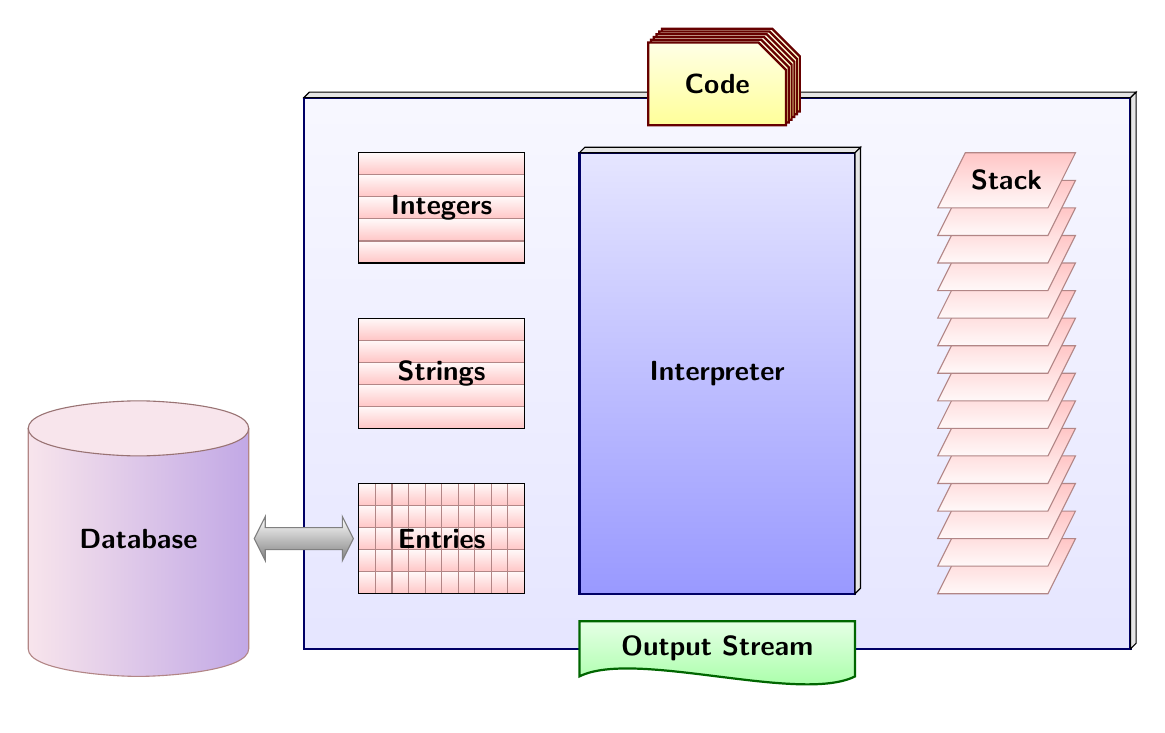
\begin{tikzpicture}[scale=.7]\sf\bfseries
  % --- bottom layer ---
  \shade[top color=white!97!blue,bottom color=white!90!blue,draw=blue!40!black,thick]
  (0,0) rectangle (15,10);
  \draw[fill=gray!20!white] (0,10) -- (.1,10.1) -- (15.1,10.1) -- (15,10) -- cycle;
  \draw[fill=gray!20!white] (15,10) -- (15.1,10.1) -- (15.1,.1) -- (15,0) -- cycle;

  % --- code ---
  \begin{scope}[shift={(6.25,9.5)},scale=.5]
    \begin{scope}[shift={(.5,.5)}]
      \shade[top color=white!90!yellow,bottom color=white!60!yellow,draw=red!40!black,thick]
      (0,0) -- (5,0) -- (5,2) -- (4,3) -- (0,3) -- cycle;
    \end{scope}
    \begin{scope}[shift={(.4,.4)}]
      \shade[top color=white!90!yellow,bottom color=white!60!yellow,draw=red!40!black,thick]
      (0,0) -- (5,0) -- (5,2) -- (4,3) -- (0,3) -- cycle;
    \end{scope}
    \begin{scope}[shift={(.3,.3)}]
      \shade[top color=white!90!yellow,bottom color=white!60!yellow,draw=red!40!black,thick]
      (0,0) -- (5,0) -- (5,2) -- (4,3) -- (0,3) -- cycle;
    \end{scope}
    \begin{scope}[shift={(.2,.2)}]
      \shade[top color=white!90!yellow,bottom color=white!60!yellow,draw=red!40!black,thick]
      (0,0) -- (5,0) -- (5,2) -- (4,3) -- (0,3) -- cycle;
    \end{scope}
    \begin{scope}[shift={(.1,.1)}]
      \shade[top color=white!90!yellow,bottom color=white!60!yellow,draw=red!40!black,thick]
      (0,0) -- (5,0) -- (5,2) -- (4,3) -- (0,3) -- cycle;
    \end{scope}
    \shade[top color=white!90!yellow,bottom color=white!60!yellow,draw=red!40!black,thick]
    (0,0) -- (5,0) -- (5,2) -- (4,3) -- (0,3) -- cycle;
  \end{scope}
  \draw (7.5,10.25) node {Code};

  % --- interpreter ---
  \shade[top color=white!90!blue,bottom color=white!60!blue,draw=blue!40!black,thick]
  (5,1) rectangle (10,9);
  \draw[fill=gray!20!white] (5,9) -- (5.1,9.1) -- (10.1,9.1) -- (10,9) -- cycle;
  \draw[fill=gray!20!white] (10,9) -- (10.1,9.1) -- (10.1,1.1) -- (10,1) -- cycle;
  \draw (7.5,5) node {Interpreter};
  
  \shade[top color=white!90!green,bottom color=white!60!green,draw=green!40!black,thick]
  (5,-.5) .. controls (6,0) and (9,-1) .. (10,-.5) -- (10,.5) -- (5,.5) -- cycle;
  \draw (7.5,0) node {Output Stream};


  % --- stack ---
  \shade[top color=white!10!pink,bottom color=white!90!pink,draw=pink!70!black,shift={(11.5,1)}] (0,0) -- (.5,1) -- (2.5,1) -- (2,0) -- cycle;
  \shade[top color=white!10!pink,bottom color=white!90!pink,draw=pink!70!black,shift={(11.5,1.5)}] (0,0) -- (.5,1) -- (2.5,1) -- (2,0) -- cycle;
  \shade[top color=white!10!pink,bottom color=white!90!pink,draw=pink!70!black,shift={(11.5,2)}] (0,0) -- (.5,1) -- (2.5,1) -- (2,0) -- cycle;
  \shade[top color=white!10!pink,bottom color=white!90!pink,draw=pink!70!black,shift={(11.5,2.5)}] (0,0) -- (.5,1) -- (2.5,1) -- (2,0) -- cycle;
  \shade[top color=white!10!pink,bottom color=white!90!pink,draw=pink!70!black,shift={(11.5,3)}] (0,0) -- (.5,1) -- (2.5,1) -- (2,0) -- cycle;
  \shade[top color=white!10!pink,bottom color=white!90!pink,draw=pink!70!black,shift={(11.5,3.5)}] (0,0) -- (.5,1) -- (2.5,1) -- (2,0) -- cycle;
  \shade[top color=white!10!pink,bottom color=white!90!pink,draw=pink!70!black,shift={(11.5,4)}] (0,0) -- (.5,1) -- (2.5,1) -- (2,0) -- cycle;
  \shade[top color=white!10!pink,bottom color=white!90!pink,draw=pink!70!black,shift={(11.5,4.5)}] (0,0) -- (.5,1) -- (2.5,1) -- (2,0) -- cycle;
  \shade[top color=white!10!pink,bottom color=white!90!pink,draw=pink!70!black,shift={(11.5,5)}] (0,0) -- (.5,1) -- (2.5,1) -- (2,0) -- cycle;
  \shade[top color=white!10!pink,bottom color=white!90!pink,draw=pink!70!black,shift={(11.5,5.5)}] (0,0) -- (.5,1) -- (2.5,1) -- (2,0) -- cycle;
  \shade[top color=white!10!pink,bottom color=white!90!pink,draw=pink!70!black,shift={(11.5,6)}] (0,0) -- (.5,1) -- (2.5,1) -- (2,0) -- cycle;
  \shade[top color=white!10!pink,bottom color=white!90!pink,draw=pink!70!black,shift={(11.5,6.5)}] (0,0) -- (.5,1) -- (2.5,1) -- (2,0) -- cycle;
  \shade[top color=white!10!pink,bottom color=white!90!pink,draw=pink!70!black,shift={(11.5,7)}] (0,0) -- (.5,1) -- (2.5,1) -- (2,0) -- cycle;
  \shade[top color=white!10!pink,bottom color=white!90!pink,draw=pink!70!black,shift={(11.5,7.5)}] (0,0) -- (.5,1) -- (2.5,1) -- (2,0) -- cycle;
  \shade[top color=white!10!pink,bottom color=white!90!pink,draw=pink!70!black,shift={(11.5,8)}] (0,0) -- (.5,1) -- (2.5,1) -- (2,0) -- cycle;
  \draw (12.75,8.5) node {Stack};

  % --- integers ---
  \shade[top color=white!90!pink,bottom color=white!10!pink,draw=pink!70!black]
  (1,7) rectangle (4,7.4);
  \shade[shift={(0,.4)},top color=white!90!pink,bottom color=white!10!pink,draw=pink!70!black]
  (1,7) rectangle (4,7.4);
  \shade[shift={(0,.8)},top color=white!90!pink,bottom color=white!10!pink,draw=pink!70!black]
  (1,7) rectangle (4,7.4);
  \shade[shift={(0,1.2)},top color=white!90!pink,bottom color=white!10!pink,draw=pink!70!black]
  (1,7) rectangle (4,7.4);
  \shade[shift={(0,1.6)},top color=white!90!pink,bottom color=white!10!pink,draw=pink!70!black]
  (1,7) rectangle (4,7.4);
  \draw (1,7) rectangle (4,9);
  \draw (2.5,8) node {Integers};

  % --- strings ---
  \shade[top color=white!90!pink,bottom color=white!10!pink,draw=pink!70!black]
  (1,4) rectangle (4,4.4);
  \shade[shift={(0,.4)},top color=white!90!pink,bottom color=white!10!pink,draw=pink!70!black]
  (1,4) rectangle (4,4.4);
  \shade[shift={(0,.8)},top color=white!90!pink,bottom color=white!10!pink,draw=pink!70!black]
  (1,4) rectangle (4,4.4);
  \shade[shift={(0,1.2)},top color=white!90!pink,bottom color=white!10!pink,draw=pink!70!black]
  (1,4) rectangle (4,4.4);
  \shade[shift={(0,1.6)},top color=white!90!pink,bottom color=white!10!pink,draw=pink!70!black]
  (1,4) rectangle (4,4.4);
  \draw (1,4) rectangle (4,6);
  \draw (2.5,5) node {Strings};

  % --- entries ---
  \shade[top color=white!90!pink,bottom color=white!10!pink,draw=pink!70!black]
  (1,1) rectangle (4,1.4);
  \shade[shift={(0,.4)},top color=white!90!pink,bottom color=white!10!pink,draw=pink!70!black]
  (1,1) rectangle (4,1.4);
  \shade[shift={(0,.8)},top color=white!90!pink,bottom color=white!10!pink,draw=pink!70!black]
  (1,1) rectangle (4,1.4);
  \shade[shift={(0,1.2)},top color=white!90!pink,bottom color=white!10!pink,draw=pink!70!black]
  (1,1) rectangle (4,1.4);
  \shade[shift={(0,1.6)},top color=white!90!pink,bottom color=white!10!pink,draw=pink!70!black]
  (1,1) rectangle (4,1.4);
  \draw[shift={(.3,0)},draw=pink!70!black] (1,1) -- (1,3);
  \draw[shift={(.6,0)},draw=pink!70!black] (1,1) -- (1,3);
  \draw[shift={(.9,0)},draw=pink!70!black] (1,1) -- (1,3);
  \draw[shift={(1.2,0)},draw=pink!70!black] (1,1) -- (1,3);
  \draw[shift={(1.5,0)},draw=pink!70!black] (1,1) -- (1,3);
  \draw[shift={(1.8,0)},draw=pink!70!black] (1,1) -- (1,3);
  \draw[shift={(2.1,0)},draw=pink!70!black] (1,1) -- (1,3);
  \draw[shift={(2.4,0)},draw=pink!70!black] (1,1) -- (1,3);
  \draw[shift={(2.7,0)},draw=pink!70!black] (1,1) -- (1,3);
  \draw (1,1) rectangle (4,3);
  \draw (2.5,2) node {Entries};

  \begin{scope}[shift={(-5,0)}]
    \shade[left color=white!96!blue!70!pink,right color=white!60!blue!60!pink,draw=pink!70!black]
    (0,0)   .. controls (0,-.4) and (1.5,-.5) ..
    (2,-.5)  .. controls (2.5,-.5) and (4,-.4) ..
    (4,0) -- (4,4) -- (0,4) -- cycle;
    \draw[shift={(0,4)},fill=white!96!blue!70!pink,draw=pink!60!black]
    (0,0)   .. controls (0,.4) and (1.5,.5) ..
    (2,.5)  .. controls (2.5,.5) and (4,.4) ..
    (4,0)   .. controls (4,-.4) and (2.5,-.5) ..
    (2,-.5) .. controls (1.5,-.5) and (0,-.4) ..
    (0,0);
  \end{scope}
  \draw (-3,2) node {Database};

%  \draw[shift={(0,-5)}]
%  (-.2,0) -- (0,.4) -- (0,.2) -- (1,.2) -- (1,.4) -- (1.2,0) --
%  (1,-.4) -- (1,-.2) -- (0,-.2) -- (0,-.4) -- cycle;

  \shade[shift={(-.7,2)}, top color=white, bottom color=gray,draw=gray]
  (-.2,0) -- (0,.4) -- (0,.2) -- (1.4,.2) -- (1.4,.4) -- (1.6,0) --
  (1.4,-.4) -- (1.4,-.2) -- (0,-.2) -- (0,-.4) -- cycle;

\end{tikzpicture}
\endgroup
\endinput
%
% Local Variables: 
% mode: latex
% TeX-master: nil
% End: 

  \caption{The BST Programming Model}
  \label{fig:bst-model}
\end{figure}


\subsection{The Database Context}

Whenever a bst program is executed a database is at hand. The program
has access to this database.

\INCOMPLETE

\subsection{Entries}

\INCOMPLETE

\subsubsection{\texttt{sort.key\$}}%
\varIndex{sort.key\$}

\INCOMPLETE


\subsection{Global Integers}

\INCOMPLETE

\subsubsection{\texttt{entry.max\$}}%
\varIndex{entry.max\$}

\INCOMPLETE
\subsubsection{\texttt{global.max\$}}%
\varIndex{global.max\$}

\INCOMPLETE

\subsection{Global Strings}

\INCOMPLETE


\section{Syntax}

The bst source code follows some very simple syntax rules. There are
only a few characters beside white-space which have a special meaning:

\begin{itemize}
\item The percent sign \verb|%| starts an endline comment (see
  section~\ref{sec:bst.comments}).
\item The double quote sign \verb|"| starts a string literal (see
  section~\ref{sec:bst.strings}).
\item The hash amrk \verb|#| starts an integer literal (see
  section~\ref{sec:bst.integers}).
\item The single quote sign \verb|'| quotes a following literal (see
  section~\ref{sec:bst.quote}).
\item The braces \verb|{| and \verb|}| enclose arguments and code (see
  section~\ref{sec:bst.code}).
\end{itemize}


\subsection{Comments}\label{sec:bst.comments}

Comments in a bst file are started with a percent sign (\verb|%|) and
continues to the end of the line. This is the same definition an in
\TeX\index{TeX@\TeX}.

The following example is taken from \File{alpha.bst}:

\begin{lstlisting}[language=bst]
  % BibTeX standard bibliography style `alpha'
\end{lstlisting}


\subsection{String Literals}\label{sec:bst.strings}

String literals in the code are enclose in double quotes '"'. The
strings contain braces only in matching pairs. As a consequence a
double quote can be included in a string by enclosing it in braces.
This is shown in the following example:

\begin{lstlisting}[language=bst,escapechar=|]
  "abc {|\char`\"|} def"
\end{lstlisting}


\subsection{Integer Literals}\label{sec:bst.integers}

Integer literals in the code are preceded by a hash mark '\#'.

\begin{lstlisting}[language=bst]
  #123
\end{lstlisting}

Integers can be negative. In this case the sign is written after the
initial hash mark:

\begin{lstlisting}[language=bst]
  #-123
\end{lstlisting}


\subsection{Quoting}\label{sec:bst.quote}

\INCOMPLETE

\begin{lstlisting}[language=bst]
  'abc
\end{lstlisting}

\subsection{Code}\label{sec:bst.code}

\INCOMPLETE

\begin{lstlisting}[language=bst]
  { skip$ }
\end{lstlisting}

\section{Expansion of Variables and Fields}

\INCOMPLETE



\section{Commands}

\subsection{\texttt{entry}}%
\cmdIndex{entry}

The declaration defines the view to an entry. For this purpose it
defines which fields are defined. In addition it defines the list of
integer entry variables and string entry variables. Thus the entry
declaration has three arguments in braces. The first one is the list
of fields the second one the list of integer entry variables and the
third the list of string entry variables. The elements of the lists
are separated by whitespace.

The fields, the entry variables and the global variables share a
common name space. Thus any name has to be unique among those.

The following example is taken from \File{alpha.bst}:

\begin{lstlisting}[language=bst]
  ENTRY
  { address
    author
    booktitle
    chapter
    edition
    editor
    howpublished
    institution
    journal
    key
    month
    note
    number
    organization
    pages
    publisher
    school
    series
    title
    type
    volume
    year
  }
  {}
  { label extra.label sort.label }
\end{lstlisting}


\subsection{\texttt{integers}}%
\cmdIndex{integers}

This declaration defines a set of global integers. It has one
argument. The argument contains a list of variable names separated by
white-space. The names must not collide with entry local strings,
entry local integers, global strings, and fields.

There may be any number of declarations of integer variables.
Nevertheless the declaration of a variable should precede its use.

The following example is taken from \File{alpha.bst}:

\begin{lstlisting}[language=bst]
  INTEGERS { output.state before.all }
\end{lstlisting}


\subsection{\texttt{strings}}
\cmdIndex{strings}

This declaration defines a set of global strings. It has one argument.
The argument contains a list of variable names separated by
white-space. The names miust not collide with entry local strings,
entry local integers, global integers, and fields.

There may be any number of declarations of string variables.
Nevertheless the declaration of a variable should precede its use.

The following example is taken from \File{alpha.bst}:

\begin{lstlisting}[language=bst]
  STRINGS { s t }
\end{lstlisting}


\subsection{\texttt{macro}}
\cmdIndex{macro}

This declaration defines a macro. It takes two arguments -- the name
of the macro and its value. The value is an expression which evaluates
to a string.

This declaration has the same effect as the definition of a macro with
the \texttt{@string} declaration in a bib file.

The following example is taken from \File{alpha.bst}:

\begin{lstlisting}[language=bst]
  MACRO {jan} {"January"}
\end{lstlisting}


\subsection{\texttt{execute}}
\cmdIndex{execute}

This command executes the function in the argument. There is no
current entry then this code is executed.

The following example is taken from \File{alpha.bst}:

\begin{lstlisting}[language=bst]
  EXECUTE {begin.bib}
\end{lstlisting}


\subsection{\texttt{iterate}}
\cmdIndex{iterate}

This command iterates over the entries in the order they are currently
in the entry list from the beginning to the end. Each entry is
considered as current entry and the function in the argument is
executed.

The following example is taken from \File{alpha.bst}:

\begin{lstlisting}[language=bst]
  ITERATE{call.type$}
\end{lstlisting}


\subsection{\texttt{reverse}}
\cmdIndex{reverse}

This command iterates over the entries in the reverse order they are
currently in the entry list from the beginning to the end. Each entry
is considered as current entry and the function in the argument is
executed.

The following example is taken from \File{alpha.bst}:

\begin{lstlisting}[language=bst]
  REVERSE{reverse.pass}
\end{lstlisting}


\subsection{\texttt{sort}}
\cmdIndex{sort}

This command sorts the entries of the database according to its sort
key lexicographically increasing. The sort key is taken from the entry
variable \texttt{sort.key\$}.

\begin{lstlisting}[language=bst]
  SORT
\end{lstlisting}


\subsection{\texttt{read}}
\cmdIndex{read}

This command read entries into the database. The database is empty
before the read command is encountered. The list of entries is ordered
according to the order they are encountered.

\begin{lstlisting}[language=bst]
  READ
\end{lstlisting}


\subsection{\texttt{function}}
\cmdIndex{function}

This declaration defines a user defined function. It takes two
arguments which are the name of the function and the code associated
with it.

\INCOMPLETE

\begin{lstlisting}[language=bst]
  FUNCTION {sortify}
  { purify$
    "l" change.case$
  }
\end{lstlisting}\fctIndex{purify\$}\fctIndex{change.case\$}


\subsection{\texttt{input}}
\cmdIndex{input}

The command takes one argument containg the name of another bst file.
This bst file is read in in place of this instruction as if the
contents of those file would have been included here. \IM{x}

If the named file or other resource could not be found then an error
is raised.

\begin{lstlisting}[language=bst]
  INPUT{some/other/bst}
\end{lstlisting}


%------------------------------------------------------------------------------
\def\BstArg#1#2#3{
  \begin{scope}[shift={(#1,#2)}]
    \shade[top color=white!10!pink,bottom color=white!90!pink,draw=pink!70!black]
    (0,0) -- (.5,1.1) -- (4.5,1.1) -- (4,0) -- cycle;
    \draw (2.25,.55) node{#3};
  \end{scope}
}%
\def\BstStream(#1)#2{
  \begin{scope}[shift={(#1)}]
    \shade[top color=white!90!green,bottom color=white!60!green,draw=green!40!black,thick]
    (5,-.5) .. controls (6,0) and (9,-1) .. (10,-.5) -- (10,.5) -- (5,.5) -- cycle;
    \draw (7.5,0) node {#2};
  \end{scope}
}%
\newenvironment{BstFunction}[1]{\bigskip\par
  \def\In##1##2{\BstArg0{##1}{##2}}%
  \def\Out##1##2{\BstArg{11}{##1}{##2}}%
  \def\Stream##1{\BstStream(12,0.5){##1}}%
  \begin{tikzpicture}[scale=.5]\sf\itshape\scriptsize
    \draw[fill=white,dashed,draw = gray]
    (0,0) -- (.5,1.1) -- (4.5,1.1) -- (4,0) -- cycle;
    \draw[gray] (2.25,.55) node{ Stack};
    % ---
    \begin{scope}[shift={(5,0)},scale=.25]
      \begin{scope}[shift={(0.5,-0.5)}]
        \draw[thick,color=white!80!gray,fill==white!70!gray]
        (0.5,1) -- (19.5,1) -- (19,0) -- (21,2) -- (21.5,4) -- (20.5,3) --
        (1.5,3) -- cycle;
      \end{scope}
      \shade[top color=white!90!gray,bottom color=white!60!gray,draw=gray!40!black,thick]
      (0.5,1) -- (19.5,1) -- (19,0) -- (21,2) -- (21.5,4) -- (20.5,3) --
      (1.5,3) -- cycle;
      \draw (11.5,5) node{#1};
    \end{scope}
    % ---
    \begin{scope}[shift={(11,0)}]
      \draw[fill=white,dashed,draw = gray]
      (0,0) -- (.5,1.1) -- (4.5,1.1) -- (4,0) -- cycle;
      \draw[gray] (2.25,.55) node{ Stack};
    \end{scope}
  }{%
  \end{tikzpicture}%
  \bigskip\par
}%


\section{Functions}

The built-in functions are the basic building blocks for user defined
functions.

\subsection{The Function \texttt{>}}%
\fctIndex{>}

This function pops two numeric arguments from the stack and
compares them. It succeeds if the first argument is less than the
second argument. In case of success the integer 1 is pushed otherwise
the integer 0.

If the stack does not contain enough items or the arguments are not
integers then an error is raised.

\begin{BstFunction}{>}
  \In1{arg2}
  \In2{arg1}
  \Out1{boolean}
\end{BstFunction}

The following example is taken from \File{alpha.bst}:

\begin{lstlisting}[language=bst]
    { namesleft #0 > }
    { 
      % some actions

      namesleft #1 - 'namesleft :=
    }
  while$
\end{lstlisting}


\subsection{The Function \texttt{<}}%
\fctIndex{<}

This function pops two numeric arguments from the stack and
compares them. It succeeds if the first argument is greater than the
second argument. In case of success the integer 1 is pushed otherwise
the integer 0.

If the stack does not contain enough items or the arguments are not
integers then an error is raised.

\begin{BstFunction}{<}
  \In1{arg2}
  \In2{arg1}
  \Out1{boolean}
\end{BstFunction}

The following example is taken from \File{alpha.bst}:

\begin{lstlisting}[language=bst]
FUNCTION {tie.or.space.connect}
{ duplicate$ text.length$ #3 <
    { "~" }
    { " " }
  if$
  swap$ * *
}
\end{lstlisting}\fctIndex{<}\fctIndex{*}%
\fctIndex{duplicate\$}\fctIndex{if\$}\fctIndex{swap\$}\fctIndex{text.length\$}


\subsection{The Function \texttt{=}}%
\fctIndex{=}

This function pops two arguments from the stack and compares them.
If the arguments are integers then it succeeds if the first argument is
equal to the second argument. If the arguments are strings then it
succeeds if both strings contain the same characters. In case of
success the integer 1 is pushed otherwise the integer 0.

If the stack does not contain enough items or the arguments have
incomparable types then an error is raised.

\begin{BstFunction}{=}
  \In1{arg2}
  \In2{arg1}
  \Out1{boolean}
\end{BstFunction}

The following example is taken from \File{alpha.bst}:

\begin{lstlisting}[language=bst]
    output.state mid.sentence =
    { "number" }
    { "Number" }
  if$
\end{lstlisting}


\subsection{The Function \texttt{+}}%
\fctIndex{+}

This function pops two numeric arguments from the stack and
pushes back the sum of the two numbers to the stack.

If the stack does not contain enough items or the arguments are not
integers then an error is raised.

\begin{BstFunction}{+}
  \In1{arg2}
  \In2{arg1}
  \Out1{sum}
\end{BstFunction}

The following example is taken from \File{alpha.bst}:

\begin{lstlisting}[language=bst]
    s len #1 +
\end{lstlisting}


\subsection{The Function \texttt{-}}%
\fctIndex{-}

This function pops two numeric arguments from the stack and
pushes back the difference of the two numbers to the stack.

If the stack does not contain enough items or the arguments are not
integers then an error is raised.

\begin{BstFunction}{-}
  \In1{arg2}
  \In2{arg1}
  \Out1{difference}
\end{BstFunction}

The following example is taken from \File{alpha.bst}:

\begin{lstlisting}[language=bst]
  namesleft #1 - 'namesleft :=
\end{lstlisting}\fctIndex{-}\fctIndex{:=}


\subsection{The Function \texttt{*}}%
\fctIndex{*}

This function takes two string arguments from the stack and pushes the
concatenated string back to the stack. If not enough arguments are on
the stack or the arguments are no strings then an error is raised.

\begin{BstFunction}{*}
  \In1{arg2}
  \In2{arg1}
  \Out1{concatenated}
\end{BstFunction}

The following example is taken from \File{alpha.bst}:

\begin{lstlisting}[language=bst]
  "there's a month but no year in " cite$ * warning$
\end{lstlisting}


\subsection{The Function \texttt{:=}}%
\fctIndex{:=}

This function assigns a value to a variable or field. It takes two
arguments from the stack. The first argument is the name of the
target. In general it needs to be quoted (see
section~\ref{sec:bst.quote}). The second argument is the appropriate
value.

\begin{BstFunction}{:=}
  \In1{value}
  \In2{name}
\end{BstFunction}

The following example is taken from \File{alpha.bst}:

\begin{lstlisting}[language=bst]
    { namesleft #0 > }
    { 
      % some actions

      namesleft #1 - 'namesleft :=
    }
  while$
\end{lstlisting}\fctIndex{>}\fctIndex{-}\fctIndex{:=}\fctIndex{while\$}


\subsection{The Function \texttt{add.period\$}}%
\fctIndex{add.period\$}

This function pops a string argument from the stack and inspects it.
It the argument ends in one of the characters period '.', exclamation
mark '!', or question mark '?' then the argument is pushed back to the
stack. Otherwise a period '.' is added to the argument and the result
pushed to the stack.

When determining the last character closing braces are ignored.

\begin{BstFunction}{add.period\$}
  \In1{string}
  \Out1{result}
\end{BstFunction}

The following example is taken from \File{alpha.bst}:

\begin{lstlisting}[language=bst]
  FUNCTION {fin.entry}
  { add.period$
    write$
    newline$
  }
\end{lstlisting}\fctIndex{add.period\$}\fctIndex{write\$}\fctIndex{newline\$}


\subsection{The Function \texttt{call.type\$}}%
\fctIndex{call.type\$}

This function looks at the current entry and calls the function
with the same name as the type. The name is normalized; i.e.
translated to lower case.

\begin{BstFunction}{call.type\$}
\end{BstFunction}

The following example is taken from \File{alpha.bst}:

\begin{lstlisting}[language=bst]
  ITERATE {call.type$}
\end{lstlisting}


\subsection{The Function \texttt{change.case\$}}%
\fctIndex{change.case\$}

This function performs case conversion. It takes two arguments from
the stack. The first argument is the format and the second argument is
the string to apply it to. The result is pushed back to the stack.

\begin{BstFunction}{change.case\$}
  \In1{format}
  \In2{string}
  \Out1{result}
\end{BstFunction}

The format controls the operation to be performed. It is a single
letter string. The following descriptions show the possibilities and
functions associated with the different format strings.

If the format is \verb|"l"| or \verb|"L"| then the string is converted
to lower case.

If the format is \verb|"u"| or \verb|"U"| then the string is converted
to upper case.

If the format is \verb|"t"| or \verb|"T"| then the string is converted
to title case.

\INCOMPLETE

If the format is not one of the legal values then a message is written
to the log stream and the input string pushed to the stack as the
result.

If the stack does not contain enough elements or the types do not
match then an error is raised.

The following example is taken from \File{alpha.bst}:

\begin{lstlisting}[language=bst]
  edition "l" change.case$
\end{lstlisting}


\subsection{The Function \texttt{chr.to.int\$}}%
\fctIndex{chr.to.int\$}

This function translates a character to the corresponding integer code
point. It takes a string argument from the stack. This argument must
contain exactly one character.

Note\IM{x} that \BibTeX~0.99c\index{BibTeX 0.99c@\BibTeX~0.99c} and
\BibTeX~8\index{BibTeX 8@\BibTeX~8} restrict the characters to 8~bit
characters. \ExBib\ has expanded the definition to 16~bit
Unicode\index{Unicode} characters.

\begin{BstFunction}{chr.to.int\$}
  \In1{character}
  \Out1{number}
\end{BstFunction}

\begin{lstlisting}[language=bst]
  "a" chr.to.int$
\end{lstlisting}


\subsection{The Function \texttt{cite\$}}%
\fctIndex{cite\$}

This function takes the citation key of the current entry and pushes
the string value to the stack. If there is no current entry then an
error is raised.

\begin{BstFunction}{cite\$}
  \Out1{key}
\end{BstFunction}

The following example is taken from \File{alpha.bst}:

\begin{lstlisting}[language=bst]
  "there's a month but no year in " cite$ * warning$
\end{lstlisting}


\subsection{The Function \texttt{duplicate\$}}%
\fctIndex{duplicate\$}

This function takes an element from the stack and pushed it back
twice. Thus the topmost element on the stack is duplicated. If the
stack is empty an error is raised.

\begin{BstFunction}{duplicate\$}
  \In1{arg}
  \Out1{arg}
  \Out2{arg}
\end{BstFunction}

\begin{lstlisting}[language=bst]
  "abc"
  duplicate$
\end{lstlisting}

\subsection{The Function \texttt{empty\$}}%
\fctIndex{empty\$}

This function pops a literal from the stack. If the argument is a
string it checks whether it contains only whitespace characters. If
the argument is a field reference it checks whether the field is
missing in the current entry. It pushes the integer 1 in case it
succeeds and 0 if it fails.

\INCOMPLETE

\begin{BstFunction}{empty\$}
  \In1{arg}
  \Out1{boolean}
\end{BstFunction}

The following example is taken from \File{alpha.bst}:

\begin{lstlisting}[language=bst]
  preamble$ empty$
    'skip$
    { preamble$ write$ newline$ }
  if$
\end{lstlisting}\fctIndex{preamble\$}\fctIndex{empty\$}\fctIndex{skip\$}%
\fctIndex{write\$}\fctIndex{newline\$}\fctIndex{if\$}


\subsection{The Function \texttt{format.name\$}}%
\fctIndex{format.name\$}

This function extracts a name from a name list and formats it. It
takes three arguments from the stack. The first argument is a format
string. It controls how the name should be formatted. The second
argument is the index of the name to be extracted. The third argument
is the name list in form of a string. The result is pushed back to the
stack.

\begin{BstFunction}{format.name\$}
  \In1{format}
  \In2{index}
  \In3{names}
  \Out1{result}
\end{BstFunction}

A name list is a string with names. The names are separated by the
word ``and'' surrounded by whitespace at brace level 0. The second
argument to the function selects which name should be formatted. The
counting of names starts with 1 for the first name.

A name may consist of the parts ``first'', ``von'', ``last'', and
``junior'' (see section~\ref{sec:names}). The format allows you to put
together those parts in various ways.


\INCOMPLETE

The following example is taken from \File{alpha.bst}:

\begin{lstlisting}[language=bst]
  editor #2 "{ff }{vv }{ll}{ jj}" format.name$
\end{lstlisting}


\subsection{The Function \texttt{if\$}}%
\fctIndex{if\$}

This function performs conditional processing. It takes three
arguments from the stack. The first argument is the else code. The
second argument is the then code and the third argument is an integer
interpreted as boolean value. If the boolean value is 0 then the else
code is executed. Otherwise the then code is executed.

The function itself does not leave anything on the stack.Nevertheless
the code executed for the branches may.

If there are less than three elements on the stack or the types do not
match then an error is raised.

\begin{BstFunction}{if\$}
  \In1{else code}
  \In2{then code}
  \In3{boolean}
\end{BstFunction}

The following example is taken from \File{alpha.bst}:

\begin{lstlisting}[language=bst]
    output.state mid.sentence =
    { "number" }
    { "Number" }
  if$
\end{lstlisting}

\subsection{The Function \texttt{int.to.chr\$}}%
\fctIndex{int.to.chr\$}

This function takes an integer code point from the stack and
translates it into a single character sting containing the character
associated to the code point. This string is left on the stack.

Note\IM{x} that \BibTeX~0.99c\index{BibTeX 0.99c@\BibTeX~0.99c} and
\BibTeX~8\index{BibTeX 8@\BibTeX~8} restrict the characters to 8~bit
characters. \ExBib\ has expanded the definition to 16~bit
Unicode\index{Unicode} characters. Thus in compatibility mode of
\ExBib\ the use of anumber larger than 255 leads to an error. In
\ExBib\ native mode those numbers are treated correctly as larger
Unicode\index{Unicode} code points.

\begin{BstFunction}{int.to.chr\$}
  \In1{number}
  \Out1{character}
\end{BstFunction}

\begin{lstlisting}[language=bst]
  #0 int.to.chr$
\end{lstlisting}

\subsection{The Function \texttt{int.to.str\$}}%
\fctIndex{int.to.str\$}

This function converts an integer to a string. It takes one integer
argument from the stack. It pushes the string consisting of the
decimal representation of the argument back to the stack.

\begin{BstFunction}{int.to.str\$}
  \In1{number}
  \Out1{string}
\end{BstFunction}

\begin{lstlisting}[language=bst]
  #123 int.to.str$
\end{lstlisting}


\subsection{The Function \texttt{missing\$}}%
\fctIndex{missing\$}

This function determines whether a field is missing. It takes one
argument from the stack. If it refers to a missing field it pushes the
integer 1 to the stack. If it refers to a defined field it pushes 0.

If the stack is empty of the argument does not refer to a field then
an error is raised.
 
\begin{BstFunction}{missing\$}
  \In1{field}
  \Out1{boolean}
\end{BstFunction}

The following example is taken from \File{alpha.bst}:

\begin{lstlisting}[language=bst]
    crossref missing$
    { "author and editor" editor either.or.check }
    'skip$
  if$
\end{lstlisting}\fctIndex{missing\$}\fctIndex{if\$}


\subsection{The Function \texttt{newline\$}}%
\fctIndex{newline\$}

This function writes a newline character to the output stream.

\begin{BstFunction}{newline\$}
  \Stream{Output Stream}
\end{BstFunction}

The following example is taken from \File{alpha.bst}:

\begin{lstlisting}[language=bst]
  "\newcommand{\etalchar}[1]{$^{#1}$}" write$ newline$
\end{lstlisting}\fctIndex{write\$}\fctIndex{newline\$}


\subsection{The Function \texttt{num.names\$}}%
\fctIndex{num.names\$}

This function takes a string argument from the stack and treats it as
a list of names. It pushes the number of names in the list as integer
to the stack.

The names are separated by the word \texttt{and}\index{and}. This word
has to be preceded and followed by whitespace characters. In addition
this word has to occur at brace level 0.

\begin{BstFunction}{num.names\$}
  \In1{names}
  \Out1{number}
\end{BstFunction}

The following example is taken from \File{alpha.bst}:

\begin{lstlisting}[language=bst]
  editor num.names$ #1 >
    { ", editors" * }
    { ", editor" * }
  if$
\end{lstlisting}\fctIndex{num.names\$}\fctIndex{>}\fctIndex{*}\fctIndex{if\$}


\subsection{The Function \texttt{pop\$}}%
\fctIndex{pop\$}

This function pops the topmost element from the stack. This element is
discarded.

\begin{BstFunction}{pop\$}
  \In1{arg}
\end{BstFunction}

The following example is taken from \File{alpha.bst}:

\begin{lstlisting}[language=bst]
FUNCTION {output}
{ duplicate$ empty$
    'pop$
    'output.nonnull
  if$
}
\end{lstlisting}\fctIndex{duplicate\$}\fctIndex{empty\$}\fctIndex{pop\$}\fctIndex{if\$}

\subsection{The Function \texttt{preamble\$}}%
\fctIndex{preamble\$}

This function takes the collected preamble from the database and
pushes it as string onto the stack.

\begin{BstFunction}{preamble\$}
  \Out1{preamble}
\end{BstFunction}

\begin{lstlisting}[language=bst]
  preamble$
\end{lstlisting}


\subsection{The Function \texttt{purify\$}}%
\fctIndex{purify\$}


\INCOMPLETE

\begin{BstFunction}{purify\$}
  \In1{string}
  \Out1{result}
\end{BstFunction}

The following example is taken from \File{alpha.bst}:

\begin{lstlisting}[language=bst]
FUNCTION {sortify}
{ purify$
  "l" change.case$
}
\end{lstlisting}\fctIndex{purify\$}\fctIndex{change.case\$}


\subsection{The Function \texttt{quote\$}}%
\fctIndex{quote\$}

This function takes no arguments it pushes a string containing the
double quote character '"' to the stack.

\begin{BstFunction}{quote\$}
  \Out1{quote}
\end{BstFunction}

This function can be used to construct a string containing a double
quote without using the brace trick:

\begin{lstlisting}[language=bst]
  "abc " quote$ * " def" * 
\end{lstlisting}\fctIndex{quote\$}\fctIndex{*}


\subsection{The Function \texttt{skip\$}}%
\fctIndex{skip\$}

This function does simply nothing. In other languages this might be
called a noop. This is useful for places where functions are
mandatory but nothing should be done.

\begin{BstFunction}{skip\$}
\end{BstFunction}

\begin{lstlisting}[language=bst]
  skip$
\end{lstlisting}


\subsection{The Function \texttt{stack\$}}%
\fctIndex{stack\$}

This function empties the stack and prints its elements to the log
file. This function is useful for debugging purposes.

\begin{BstFunction}{stack\$}
  \In1{...}
  \In2{...}
  \Out0{Empty}
\end{BstFunction}

\begin{lstlisting}[language=bst]
  stack$
\end{lstlisting}


\subsection{The Function \texttt{substring\$}}%
\fctIndex{substring\$}

This function computes the substring of a string. It takes three
arguments from the stack. The first argument is an integer denoting
the maximal length of the substring. At most this many character units
will be extracted.

The second argument is the start index of the substring -- an integer.
If start is positive then the first characters are extracted.  The
index 1 denotes the first character. If start is negative then the
last characters are extracted.  The index -1 denotes the last
character.

The third argument is the string to take the substring from. The
string is interpreted taking blocks in braces into account. A block in
braces counts as one character unit. Thus it is guaranteed that blocks
-- which have a special meaning in \TeX\index{TeX@\TeX} and
\LaTeX\index{LaTeX@\LaTeX} -- are never broken.

The resulting substring is pushed back to the stack.

If the stack has less than three arguments when the function is
invoked or the types of the arguments do not fit then an error is
raised.

\begin{BstFunction}{substring\$}
  \In1{string}
  \In2{start}
  \In3{length}
  \Out0{substring}
\end{BstFunction}

\begin{lstlisting}[language=bst]
  cite$ #1 #3 substring$
\end{lstlisting}

\subsection{The Function \texttt{swap\$}}%
\fctIndex{swap\$}

This function takes the two topmost elements from the stack and
exchanges their order on the stack. This means that the topmost
element becomes the second one and the second element becomes the
topmost one. The elements can be of any type.

If there are less than two elements on the stack then an error is
raised.

\begin{BstFunction}{swap\$}
  \In1{arg1}
  \In2{arg2}
  \Out1{arg2}
  \Out2{arg1}
\end{BstFunction}

\begin{lstlisting}[language=bst]
  swap$
\end{lstlisting}


\subsection{The Function \texttt{text.length\$}}%
\fctIndex{text.length\$}

This function computes the length of a text. The length is the number
of character units.

\INCOMPLETE

\begin{BstFunction}{text.length\$}
  \In1{text}
  \Out1{length}
\end{BstFunction}

\begin{lstlisting}[language=bst]
  preamble$ text.length$
\end{lstlisting}


\subsection{The Function \texttt{text.prefix\$}}%
\fctIndex{text.prefix\$}

\INCOMPLETE

\begin{BstFunction}{text.prefix\$}
  \In1{text}
  \In2{length}
  \Out1{prefix}
\end{BstFunction}

The following example is taken from \File{alpha.bst}:

\begin{lstlisting}[language=bst]
  key #3 text.prefix$
\end{lstlisting}\fctIndex{text.prefix\$}


\subsection{The Function \texttt{top\$}}%
\fctIndex{top\$}

This function pops the topmost literal from the stack and prints it
to the log stream. This function is meant for debugging purposes.
If the stack is empty an error is raised.

\begin{BstFunction}{top\$}
  \In1{argument}
\end{BstFunction}

\begin{lstlisting}[language=bst]
  top$
\end{lstlisting}


\subsection{The Function \texttt{type\$}}%
\fctIndex{type\$}

If the function is executed in the context of a current entry the type
of this entry is pushed to the stack as a string. The type is always
normalized by translating all characters to lower case.

If the function is executed outside the scope of a current entry then
the empty string is pushed to the stack.

\begin{BstFunction}{type\$}
  \Out1{type}
\end{BstFunction}

The following example is taken from \File{alpha.bst}:

\begin{lstlisting}[language=bst]
  type$ "book" =
  type$ "inbook" =
  or
\end{lstlisting}\fctIndex{=}


\subsection{The Function \texttt{warning\$}}%
\fctIndex{warning\$}

This function pops a string from the stack and prints it as a
warning to the log stream. The message is terminated by a newline character.

The line in the log file may be rewrapped to fit into a given line
length.

An empty stack leads to an error as well as a wrong type argument on
the stack.

\begin{BstFunction}{warning\$}
  \In1{message}
  \Stream{Log Stream}
\end{BstFunction}

The following example is taken from \File{alpha.bst}:

\begin{lstlisting}[language=bst]
  "there's a number but no series in " cite$ * warning$ 
\end{lstlisting}%
\fctIndex{cite\$}\fctIndex{warning\$}


\subsection{The Function \texttt{while\$}}%
\fctIndex{while\$}

This function is a loop construction. It takes two arguments form the
stack. Both of them are code segments. The first argument is code to
be executed repeatedly. The second argument is a conditional. The
conditional is executed. If the topmost element of the stack is
numeric and not 0 then the first argument is executed and the process
is repeated.

If the stack has less than two elements, the elements are of the
wrong type, or the conditional does not leave a number on the stack
then an error is raised.

\begin{BstFunction}{while\$}
  \In1{code}
  \In2{condition}
\end{BstFunction}

The following example is taken from \File{alpha.bst}:

\begin{lstlisting}[language=bst]
    { namesleft #0 > }
    { s nameptr "{ff~}{vv~}{ll}{, jj}" format.name$ 't :=

      % some more action

      nameptr #1 + 'nameptr :=
      namesleft #1 - 'namesleft :=
    }
  while$
\end{lstlisting}%
\fctIndex{while\$}\fctIndex{format.name\$}\fctIndex{+}\fctIndex{-}\fctIndex{>}%
\fctIndex{:=}


\subsection{The Function \texttt{width\$}}%
\fctIndex{width\$}

This function pops a string from the stack and tries to compute the
width of the string when typeset. For this purpose the width of the
characters in the font cmr10 are used. Some control sequences are
treated specially.

\begin{BstFunction}{width\$}
  \In1{argument}
  \Out1{width}
\end{BstFunction}

The following example is taken from \File{alpha.bst}:

\begin{lstlisting}[language=bst]
  label width$
\end{lstlisting}


\subsection{The Function \texttt{write\$}}%
\fctIndex{write\$}

This function pops a string from the stack and prints it as a
message to the output stream.

\begin{BstFunction}{write\$}
  \In1{message}
  \Stream{Output Stream}
\end{BstFunction}

The following example is taken from \File{alpha.bst}:

\begin{lstlisting}[language=bst]
  "\end{thebibliography}" write$
\end{lstlisting}

\index{BST language|)}%
\endinput
%
% Local Variables: 
% mode: latex
% TeX-master: "exbib-users"
% End: 

%%*****************************************************************************
%% Copyright (c) 2008-2010 Gerd Neugebauer
%%
%% Permission is granted to copy, distribute and/or modify this document
%% under the terms of the GNU Free Documentation License, Version 1.2
%% or any later version published by the Free Software Foundation;
%% with no Invariant Sections, no Front-Cover Texts, and no Back-Cover Texts.
%%
%%*****************************************************************************
%% $Id:csf.tex 7067 2008-05-18 11:06:56Z gene $
%%*****************************************************************************
%% Author: Gerd Neugebauer
%%-----------------------------------------------------------------------------

\section{CSF}%
\label{sec:csf}%
\index{csf|(}

One problem of the original \BibTeX~0.99c is the restriction to 7 bit
characters. To solve this problem the cs files have been introduced in
\BibTeX~8\index{BibTeX 8|\BibTeX 8}:
\IM{8x}

\begin{verbatim}
  sort=csf
\end{verbatim}

\begin{verbatim}
  sort=csf:resource
\end{verbatim}

\INCOMPLETE

\index{csf|)}

\endinput
%
% Local Variables: 
% mode: latex
% TeX-master: "../exbib-manual"
% End: 


\appendix
%%*****************************************************************************
%% $Id$
%%*****************************************************************************
%% Author: Gerd Neugebauer
%%-----------------------------------------------------------------------------
\chapter{Licenses}%
\index{license|(}%
%---------The file header---------------------------------------------
%\documentclass[a4paper,12pt]{book} % possibilities : report book article , etc.
%
%\usepackage[english]{babel} %language selection
%\usepackage[T1]{fontenc}
%
%\pagenumbering{arabic}
%
%\usepackage{hyperref}
%\hypersetup{colorlinks, 
%           citecolor=black,
%           filecolor=black,
%           linkcolor=black,
%           urlcolor=black,
%           pdftex}
%
%           
%\begin{document}
%---------------------------------------------------------------------
\section{GNU Free Documentation License}
\label{label_fdl}

\begin{multicols}{3}\tiny\sf%\scriptsize

 \begin{center}

   Version 1.2, November 2002

   Copyright \copyright\ 2000,2001,2002  Free Software Foundation, Inc.
 
   \bigskip
 
   51 Franklin St, Fifth Floor, Boston, MA  02110-1301  USA
  
   \bigskip
 
   Everyone is permitted to copy and distribute verbatim copies
   of this license document, but changing it is not allowed.
\end{center}


\begin{center}
{\bf Preamble}
\end{center}

The purpose of this License is to make a manual, textbook, or other
functional and useful document ``free'' in the sense of freedom: to
assure everyone the effective freedom to copy and redistribute it,
with or without modifying it, either commercially or noncommercially.
Secondarily, this License preserves for the author and publisher a way
to get credit for their work, while not being considered responsible
for modifications made by others.

This License is a kind of ``copyleft'', which means that derivative
works of the document must themselves be free in the same sense.  It
complements the GNU General Public License, which is a copyleft
license designed for free software.

We have designed this License in order to use it for manuals for free
software, because free software needs free documentation: a free
program should come with manuals providing the same freedoms that the
software does.  But this License is not limited to software manuals;
it can be used for any textual work, regardless of subject matter or
whether it is published as a printed book.  We recommend this License
principally for works whose purpose is instruction or reference.


\begin{center}
{\bf 1. APPLICABILITY AND DEFINITIONS}
%\addcontentsline{toc}{section}{1. APPLICABILITY AND DEFINITIONS}
\end{center}

This License applies to any manual or other work, in any medium, that
contains a notice placed by the copyright holder saying it can be
distributed under the terms of this License.  Such a notice grants a
world-wide, royalty-free license, unlimited in duration, to use that
work under the conditions stated herein.  The \textbf{``Document''}, below,
refers to any such manual or work.  Any member of the public is a
licensee, and is addressed as \textbf{``you''}.  You accept the license if you
copy, modify or distribute the work in a way requiring permission
under copyright law.

A \textbf{``Modified Version''} of the Document means any work containing the
Document or a portion of it, either copied verbatim, or with
modifications and/or translated into another language.

A \textbf{``Secondary Section''} is a named appendix or a front-matter section of
the Document that deals exclusively with the relationship of the
publishers or authors of the Document to the Document's overall subject
(or to related matters) and contains nothing that could fall directly
within that overall subject.  (Thus, if the Document is in part a
textbook of mathematics, a Secondary Section may not explain any
mathematics.)  The relationship could be a matter of historical
connection with the subject or with related matters, or of legal,
commercial, philosophical, ethical or political position regarding
them.

The \textbf{``Invariant Sections''} are certain Secondary Sections whose titles
are designated, as being those of Invariant Sections, in the notice
that says that the Document is released under this License.  If a
section does not fit the above definition of Secondary then it is not
allowed to be designated as Invariant.  The Document may contain zero
Invariant Sections.  If the Document does not identify any Invariant
Sections then there are none.

The \textbf{``Cover Texts''} are certain short passages of text that are listed,
as Front-Cover Texts or Back-Cover Texts, in the notice that says that
the Document is released under this License.  A Front-Cover Text may
be at most 5 words, and a Back-Cover Text may be at most 25 words.

A \textbf{``Transparent''} copy of the Document means a machine-readable copy,
represented in a format whose specification is available to the
general public, that is suitable for revising the document
straightforwardly with generic text editors or (for images composed of
pixels) generic paint programs or (for drawings) some widely available
drawing editor, and that is suitable for input to text formatters or
for automatic translation to a variety of formats suitable for input
to text formatters.  A copy made in an otherwise Transparent file
format whose markup, or absence of markup, has been arranged to thwart
or discourage subsequent modification by readers is not Transparent.
An image format is not Transparent if used for any substantial amount
of text.  A copy that is not ``Transparent'' is called \textbf{``Opaque''}.

Examples of suitable formats for Transparent copies include plain
ASCII without markup, Texinfo input format, \LaTeX\ input format, SGML
or XML using a publicly available DTD, and standard-conforming simple
HTML, PostScript or PDF designed for human modification.  Examples of
transparent image formats include PNG, XCF and JPG.  Opaque formats
include proprietary formats that can be read and edited only by
proprietary word processors, SGML or XML for which the DTD and/or
processing tools are not generally available, and the
machine-generated HTML, PostScript or PDF produced by some word
processors for output purposes only.

The \textbf{``Title Page''} means, for a printed book, the title page itself,
plus such following pages as are needed to hold, legibly, the material
this License requires to appear in the title page.  For works in
formats which do not have any title page as such, ``Title Page'' means
the text near the most prominent appearance of the work's title,
preceding the beginning of the body of the text.

A section \textbf{``Entitled XYZ''} means a named subunit of the Document whose
title either is precisely XYZ or contains XYZ in parentheses following
text that translates XYZ in another language.  (Here XYZ stands for a
specific section name mentioned below, such as \textbf{``Acknowledgements''},
\textbf{``Dedications''}, \textbf{``Endorsements''}, or \textbf{``History''}.)  
To \textbf{``Preserve the Title''}
of such a section when you modify the Document means that it remains a
section ``Entitled XYZ'' according to this definition.

The Document may include Warranty Disclaimers next to the notice which
states that this License applies to the Document.  These Warranty
Disclaimers are considered to be included by reference in this
License, but only as regards disclaiming warranties: any other
implication that these Warranty Disclaimers may have is void and has
no effect on the meaning of this License.


\begin{center}
{\bf 2. VERBATIM COPYING}
%\addcontentsline{toc}{section}{2. VERBATIM COPYING}
\end{center}

You may copy and distribute the Document in any medium, either
commercially or noncommercially, provided that this License, the
copyright notices, and the license notice saying this License applies
to the Document are reproduced in all copies, and that you add no other
conditions whatsoever to those of this License.  You may not use
technical measures to obstruct or control the reading or further
copying of the copies you make or distribute.  However, you may accept
compensation in exchange for copies.  If you distribute a large enough
number of copies you must also follow the conditions in section 3.

You may also lend copies, under the same conditions stated above, and
you may publicly display copies.


\begin{center}
{\bf 3. COPYING IN QUANTITY}
%\addcontentsline{toc}{section}{3. COPYING IN QUANTITY}
\end{center}


If you publish printed copies (or copies in media that commonly have
printed covers) of the Document, numbering more than 100, and the
Document's license notice requires Cover Texts, you must enclose the
copies in covers that carry, clearly and legibly, all these Cover
Texts: Front-Cover Texts on the front cover, and Back-Cover Texts on
the back cover.  Both covers must also clearly and legibly identify
you as the publisher of these copies.  The front cover must present
the full title with all words of the title equally prominent and
visible.  You may add other material on the covers in addition.
Copying with changes limited to the covers, as long as they preserve
the title of the Document and satisfy these conditions, can be treated
as verbatim copying in other respects.

If the required texts for either cover are too voluminous to fit
legibly, you should put the first ones listed (as many as fit
reasonably) on the actual cover, and continue the rest onto adjacent
pages.

If you publish or distribute Opaque copies of the Document numbering
more than 100, you must either include a machine-readable Transparent
copy along with each Opaque copy, or state in or with each Opaque copy
a computer-network location from which the general network-using
public has access to download using public-standard network protocols
a complete Transparent copy of the Document, free of added material.
If you use the latter option, you must take reasonably prudent steps,
when you begin distribution of Opaque copies in quantity, to ensure
that this Transparent copy will remain thus accessible at the stated
location until at least one year after the last time you distribute an
Opaque copy (directly or through your agents or retailers) of that
edition to the public.

It is requested, but not required, that you contact the authors of the
Document well before redistributing any large number of copies, to give
them a chance to provide you with an updated version of the Document.


\begin{center}
{\bf 4. MODIFICATIONS}
%\addcontentsline{toc}{section}{4. MODIFICATIONS}
\end{center}

You may copy and distribute a Modified Version of the Document under
the conditions of sections 2 and 3 above, provided that you release
the Modified Version under precisely this License, with the Modified
Version filling the role of the Document, thus licensing distribution
and modification of the Modified Version to whoever possesses a copy
of it.  In addition, you must do these things in the Modified Version:

\begin{itemize}
\item[A.] 
   Use in the Title Page (and on the covers, if any) a title distinct
   from that of the Document, and from those of previous versions
   (which should, if there were any, be listed in the History section
   of the Document).  You may use the same title as a previous version
   if the original publisher of that version gives permission.
   
\item[B.]
   List on the Title Page, as authors, one or more persons or entities
   responsible for authorship of the modifications in the Modified
   Version, together with at least five of the principal authors of the
   Document (all of its principal authors, if it has fewer than five),
   unless they release you from this requirement.
   
\item[C.]
   State on the Title page the name of the publisher of the
   Modified Version, as the publisher.
   
\item[D.]
   Preserve all the copyright notices of the Document.
   
\item[E.]
   Add an appropriate copyright notice for your modifications
   adjacent to the other copyright notices.
   
\item[F.]
   Include, immediately after the copyright notices, a license notice
   giving the public permission to use the Modified Version under the
   terms of this License, in the form shown in the Addendum below.
   
\item[G.]
   Preserve in that license notice the full lists of Invariant Sections
   and required Cover Texts given in the Document's license notice.
   
\item[H.]
   Include an unaltered copy of this License.
   
\item[I.]
   Preserve the section Entitled ``History'', Preserve its Title, and add
   to it an item stating at least the title, year, new authors, and
   publisher of the Modified Version as given on the Title Page.  If
   there is no section Entitled ``History'' in the Document, create one
   stating the title, year, authors, and publisher of the Document as
   given on its Title Page, then add an item describing the Modified
   Version as stated in the previous sentence.
   
\item[J.]
   Preserve the network location, if any, given in the Document for
   public access to a Transparent copy of the Document, and likewise
   the network locations given in the Document for previous versions
   it was based on.  These may be placed in the ``History'' section.
   You may omit a network location for a work that was published at
   least four years before the Document itself, or if the original
   publisher of the version it refers to gives permission.
   
\item[K.]
   For any section Entitled ``Acknowledgements'' or ``Dedications'',
   Preserve the Title of the section, and preserve in the section all
   the substance and tone of each of the contributor acknowledgements
   and/or dedications given therein.
   
\item[L.]
   Preserve all the Invariant Sections of the Document,
   unaltered in their text and in their titles.  Section numbers
   or the equivalent are not considered part of the section titles.
   
\item[M.]
   Delete any section Entitled ``Endorsements''.  Such a section
   may not be included in the Modified Version.
   
\item[N.]
   Do not retitle any existing section to be Entitled ``Endorsements''
   or to conflict in title with any Invariant Section.
   
\item[O.]
   Preserve any Warranty Disclaimers.
\end{itemize}

If the Modified Version includes new front-matter sections or
appendices that qualify as Secondary Sections and contain no material
copied from the Document, you may at your option designate some or all
of these sections as invariant.  To do this, add their titles to the
list of Invariant Sections in the Modified Version's license notice.
These titles must be distinct from any other section titles.

You may add a section Entitled ``Endorsements'', provided it contains
nothing but endorsements of your Modified Version by various
parties--for example, statements of peer review or that the text has
been approved by an organization as the authoritative definition of a
standard.

You may add a passage of up to five words as a Front-Cover Text, and a
passage of up to 25 words as a Back-Cover Text, to the end of the list
of Cover Texts in the Modified Version.  Only one passage of
Front-Cover Text and one of Back-Cover Text may be added by (or
through arrangements made by) any one entity.  If the Document already
includes a cover text for the same cover, previously added by you or
by arrangement made by the same entity you are acting on behalf of,
you may not add another; but you may replace the old one, on explicit
permission from the previous publisher that added the old one.

The author(s) and publisher(s) of the Document do not by this License
give permission to use their names for publicity for or to assert or
imply endorsement of any Modified Version.


\begin{center}
{\bf 5. COMBINING DOCUMENTS}
%\addcontentsline{toc}{section}{5. COMBINING DOCUMENTS}
\end{center}


You may combine the Document with other documents released under this
License, under the terms defined in section 4 above for modified
versions, provided that you include in the combination all of the
Invariant Sections of all of the original documents, unmodified, and
list them all as Invariant Sections of your combined work in its
license notice, and that you preserve all their Warranty Disclaimers.

The combined work need only contain one copy of this License, and
multiple identical Invariant Sections may be replaced with a single
copy.  If there are multiple Invariant Sections with the same name but
different contents, make the title of each such section unique by
adding at the end of it, in parentheses, the name of the original
author or publisher of that section if known, or else a unique number.
Make the same adjustment to the section titles in the list of
Invariant Sections in the license notice of the combined work.

In the combination, you must combine any sections Entitled ``History''
in the various original documents, forming one section Entitled
``History''; likewise combine any sections Entitled ``Acknowledgements'',
and any sections Entitled ``Dedications''.  You must delete all sections
Entitled ``Endorsements''.

\begin{center}
{\bf 6. COLLECTIONS OF DOCUMENTS}
%\addcontentsline{toc}{section}{6. COLLECTIONS OF DOCUMENTS}
\end{center}

You may make a collection consisting of the Document and other documents
released under this License, and replace the individual copies of this
License in the various documents with a single copy that is included in
the collection, provided that you follow the rules of this License for
verbatim copying of each of the documents in all other respects.

You may extract a single document from such a collection, and distribute
it individually under this License, provided you insert a copy of this
License into the extracted document, and follow this License in all
other respects regarding verbatim copying of that document.


\begin{center}
{\bf 7. AGGREGATION WITH INDEPENDENT WORKS}
%\addcontentsline{toc}{section}{7. AGGREGATION WITH INDEPENDENT WORKS}
\end{center}


A compilation of the Document or its derivatives with other separate
and independent documents or works, in or on a volume of a storage or
distribution medium, is called an ``aggregate'' if the copyright
resulting from the compilation is not used to limit the legal rights
of the compilation's users beyond what the individual works permit.
When the Document is included in an aggregate, this License does not
apply to the other works in the aggregate which are not themselves
derivative works of the Document.

If the Cover Text requirement of section 3 is applicable to these
copies of the Document, then if the Document is less than one half of
the entire aggregate, the Document's Cover Texts may be placed on
covers that bracket the Document within the aggregate, or the
electronic equivalent of covers if the Document is in electronic form.
Otherwise they must appear on printed covers that bracket the whole
aggregate.


\begin{center}
{\bf 8. TRANSLATION}
%\addcontentsline{toc}{section}{8. TRANSLATION}
\end{center}


Translation is considered a kind of modification, so you may
distribute translations of the Document under the terms of section 4.
Replacing Invariant Sections with translations requires special
permission from their copyright holders, but you may include
translations of some or all Invariant Sections in addition to the
original versions of these Invariant Sections.  You may include a
translation of this License, and all the license notices in the
Document, and any Warranty Disclaimers, provided that you also include
the original English version of this License and the original versions
of those notices and disclaimers.  In case of a disagreement between
the translation and the original version of this License or a notice
or disclaimer, the original version will prevail.

If a section in the Document is Entitled ``Acknowledgements'',
``Dedications'', or ``History'', the requirement (section 4) to Preserve
its Title (section 1) will typically require changing the actual
title.


\begin{center}
{\bf 9. TERMINATION}
%\addcontentsline{toc}{section}{9. TERMINATION}
\end{center}


You may not copy, modify, sublicense, or distribute the Document except
as expressly provided for under this License.  Any other attempt to
copy, modify, sublicense or distribute the Document is void, and will
automatically terminate your rights under this License.  However,
parties who have received copies, or rights, from you under this
License will not have their licenses terminated so long as such
parties remain in full compliance.


\begin{center}
{\bf 10. FUTURE REVISIONS OF THIS LICENSE}
%\addcontentsline{toc}{section}{10. FUTURE REVISIONS OF THIS LICENSE}
\end{center}


The Free Software Foundation may publish new, revised versions
of the GNU Free Documentation License from time to time.  Such new
versions will be similar in spirit to the present version, but may
differ in detail to address new problems or concerns.  See
\url{http://www.gnu.org/copyleft/}.

Each version of the License is given a distinguishing version number.
If the Document specifies that a particular numbered version of this
License ``or any later version'' applies to it, you have the option of
following the terms and conditions either of that specified version or
of any later version that has been published (not as a draft) by the
Free Software Foundation.  If the Document does not specify a version
number of this License, you may choose any version ever published (not
as a draft) by the Free Software Foundation.


\begin{center}
{\bf ADDENDUM: How to use this License for your documents}
%\addcontentsline{toc}{section}{ADDENDUM: How to use this License for your documents}
\end{center}

To use this License in a document you have written, include a copy of
the License in the document and put the following copyright and
license notices just after the title page:

%\bigskip
\begin{quote}
    Copyright \copyright  YEAR  YOUR NAME.\\
    Permission is granted to copy, distribute and/or modify this document
    under the terms of the GNU Free Documentation License, Version 1.2
    or any later version published by the Free Software Foundation;
    with no Invariant Sections, no Front-Cover Texts, and no Back-Cover Texts.
    A copy of the license is included in the section entitled ``GNU
    Free Documentation License''.
\end{quote}
%\bigskip
    
If you have Invariant Sections, Front-Cover Texts and Back-Cover Texts,
replace the ``with\dots Texts.'' line with this:

%\bigskip
\begin{quote}
    with the Invariant Sections being LIST THEIR TITLES, with the
    Front-Cover Texts being LIST, and with the Back-Cover Texts being LIST.
\end{quote}
%\bigskip
    
If you have Invariant Sections without Cover Texts, or some other
combination of the three, merge those two alternatives to suit the
situation.

If your document contains nontrivial examples of program code, we
recommend releasing these examples in parallel under your choice of
free software license, such as the GNU General Public License,
to permit their use in free software.

%---------------------------------------------------------------------
%\end{document}
\end{multicols}


\section{GNU Library General Public License}

\begin{multicols}{3}\tiny\sf%\scriptsize

\begin{center}
  Version 2, June 1991 
\end{center}

Copyright \copyright\ 1991 Free Software Foundation, Inc.
59 Temple Place - Suite 330, Boston, MA  02111-1307, USA
Everyone is permitted to copy and distribute verbatim copies
of this license document, but changing it is not allowed.

[This is the first released version of the library GPL.  It is
 numbered 2 because it goes with version 2 of the ordinary GPL.]

\begin{center}
\bf Preamble
\end{center}

The licenses for most software are designed to take away your freedom to
share and change it. By contrast, the GNU General Public Licenses are
intended to guarantee your freedom to share and change free software--to
make sure the software is free for all its users.

This license, the Library General Public License, applies to some specially
designated Free Software Foundation software, and to any other libraries
whose authors decide to use it. You can use it for your libraries, too.

When we speak of free software, we are referring to freedom, not price. Our
General Public Licenses are designed to make sure that you have the freedom
to distribute copies of free software (and charge for this service if you
wish), that you receive source code or can get it if you want it, that you
can change the software or use pieces of it in new free programs; and that
you know you can do these things.

To protect your rights, we need to make restrictions that forbid anyone to
deny you these rights or to ask you to surrender the rights. These
restrictions translate to certain responsibilities for you if you
distribute copies of the library, or if you modify it.

For example, if you distribute copies of the library, whether gratis or for
a fee, you must give the recipients all the rights that we gave you. You
must make sure that they, too, receive or can get the source code. If you
link a program with the library, you must provide complete object files to
the recipients so that they can relink them with the library, after making
changes to the library and recompiling it. And you must show them these
terms so they know their rights.

Our method of protecting your rights has two steps: (1) copyright the
library, and (2) offer you this license which gives you legal permission to
copy, distribute and/or modify the library.

Also, for each distributor's protection, we want to make certain that
everyone understands that there is no warranty for this free library. If
the library is modified by someone else and passed on, we want its
recipients to know that what they have is not the original version, so that
any problems introduced by others will not reflect on the original authors'
reputations.

Finally, any free program is threatened constantly by software patents. We
wish to avoid the danger that companies distributing free software will
individually obtain patent licenses, thus in effect transforming the
program into proprietary software. To prevent this, we have made it clear
that any patent must be licensed for everyone's free use or not licensed at
all.

Most GNU software, including some libraries, is covered by the ordinary GNU
General Public License, which was designed for utility programs. This
license, the GNU Library General Public License, applies to certain
designated libraries. This license is quite different from the ordinary
one; be sure to read it in full, and don't assume that anything in it is
the same as in the ordinary license.

The reason we have a separate public license for some libraries is that
they blur the distinction we usually make between modifying or adding to a
program and simply using it. Linking a program with a library, without
changing the library, is in some sense simply using the library, and is
analogous to running a utility program or application program. However, in
a textual and legal sense, the linked executable is a combined work, a
derivative of the original library, and the ordinary General Public License
treats it as such.

Because of this blurred distinction, using the ordinary General Public
License for libraries did not effectively promote software sharing, because
most developers did not use the libraries. We concluded that weaker
conditions might promote sharing better.

However, unrestricted linking of non-free programs would deprive the users
of those programs of all benefit from the free status of the libraries
themselves. This Library General Public License is intended to permit
developers of non-free programs to use free libraries, while preserving
your freedom as a user of such programs to change the free libraries that
are incorporated in them. (We have not seen how to achieve this as regards
changes in header files, but we have achieved it as regards changes in the
actual functions of the Library.) The hope is that this will lead to faster
development of free libraries.

The precise terms and conditions for copying, distribution and modification
follow. Pay close attention to the difference between a ``work based on the
library'' and a ``work that uses the library''. The former contains code
derived from the library, while the latter only works together with the
library.

Note that it is possible for a library to be covered by the ordinary
General Public License rather than by this special one.

\begin{center}
\bf TERMS AND CONDITIONS FOR COPYING, DISTRIBUTION AND MODIFICATION
\end{center}

\begin{itemize}
\item[0.] This License Agreement applies to any software library which
  contains a notice placed by the copyright holder or other authorized
  party saying it may be distributed under the terms of this Library
  General Public License (also called ``this License''). Each licensee
  is addressed as ``you''.

   A ``library'' means a collection of software functions and/or data
   prepared so as to be conveniently linked with application programs
   (which use some of those functions and data) to form executables.

   The ``Library'', below, refers to any such software library or work which
   has been distributed under these terms. A ``work based on the Library''
   means either the Library or any derivative work under copyright law:
   that is to say, a work containing the Library or a portion of it, either
   verbatim or with modifications and/or translated straightforwardly into
   another language. (Hereinafter, translation is included without
   limitation in the term ``modification''.)

   ``Source code'' for a work means the preferred form of the work for making
   modifications to it. For a library, complete source code means all the
   source code for all modules it contains, plus any associated interface
   definition files, plus the scripts used to control compilation and
   installation of the library.

   Activities other than copying, distribution and modification are not
   covered by this License; they are outside its scope. The act of running
   a program using the Library is not restricted, and output from such a
   program is covered only if its contents constitute a work based on the
   Library (independent of the use of the Library in a tool for writing
   it). Whether that is true depends on what the Library does and what the
   program that uses the Library does.
   
 \item[1.] You may copy and distribute verbatim copies of the
   Library's complete source code as you receive it, in any medium,
   provided that you conspicuously and appropriately publish on each
   copy an appropriate copyright notice and disclaimer of warranty;
   keep intact all the notices that refer to this License and to the
   absence of any warranty; and distribute a copy of this License
   along with the Library.

   You may charge a fee for the physical act of transferring a copy, and
   you may at your option offer warranty protection in exchange for a fee.
   
 \item[2.] You may modify your copy or copies of the Library or any
   portion of it, thus forming a work based on the Library, and copy
   and distribute such modifications or work under the terms of
   Section 1 above, provided that you also meet all of these
   conditions:

   \begin{itemize}
   \item[a)] The modified work must itself be a software library.
     
   \item[b)] You must cause the files modified to carry prominent
     notices stating that you changed the files and the date of any
     change.
     
   \item[c)] You must cause the whole of the work to be licensed at no
     charge to all third parties under the terms of this License.
     
   \item[d)] If a facility in the modified Library refers to a
     function or a table of data to be supplied by an application
     program that uses the facility, other than as an argument passed
     when the facility is invoked, then you must make a good faith
     effort to ensure that, in the event an application does not
     supply such function or table, the facility still operates, and
     performs whatever part of its purpose remains meaningful. (For
     example, a function in a library to compute square roots has a
     purpose that is entirely well-defined independent of the
     application. Therefore, Subsection 2d requires that any
     application-supplied function or table used by this function must
     be optional: if the application does not supply it, the square
     root function must still compute square roots.)
   \end{itemize}

   These requirements apply to the modified work as a whole. If
   identifiable sections of that work are not derived from the Library, and
   can be reasonably considered independent and separate works in
   themselves, then this License, and its terms, do not apply to those
   sections when you distribute them as separate works. But when you
   distribute the same sections as part of a whole which is a work based on
   the Library, the distribution of the whole must be on the terms of this
   License, whose permissions for other licensees extend to the entire
   whole, and thus to each and every part regardless of who wrote it.

   Thus, it is not the intent of this section to claim rights or contest
   your rights to work written entirely by you; rather, the intent is to
   exercise the right to control the distribution of derivative or
   collective works based on the Library.

   In addition, mere aggregation of another work not based on the Library
   with the Library (or with a work based on the Library) on a volume of a
   storage or distribution medium does not bring the other work under the
   scope of this License.
   
 \item[3.] You may opt to apply the terms of the ordinary GNU General
   Public License instead of this License to a given copy of the
   Library. To do this, you must alter all the notices that refer to
   this License, so that they refer to the ordinary GNU General Public
   License, version 2, instead of to this License. (If a newer version
   than version 2 of the ordinary GNU General Public License has
   appeared, then you can specify that version instead if you wish.)
   Do not make any other change in these notices.

   Once this change is made in a given copy, it is irreversible for that
   copy, so the ordinary GNU General Public License applies to all
   subsequent copies and derivative works made from that copy.

   This option is useful when you wish to copy part of the code of the
   Library into a program that is not a library.
   
 \item[4.] You may copy and distribute the Library (or a portion or
   derivative of it, under Section 2) in object code or executable
   form under the terms of Sections 1 and 2 above provided that you
   accompany it with the complete corresponding machine-readable
   source code, which must be distributed under the terms of Sections
   1 and 2 above on a medium customarily used for software
   interchange.

   If distribution of object code is made by offering access to copy from a
   designated place, then offering equivalent access to copy the source
   code from the same place satisfies the requirement to distribute the
   source code, even though third parties are not compelled to copy the
   source along with the object code.
   
 \item[5.] A program that contains no derivative of any portion of the
   Library, but is designed to work with the Library by being compiled
   or linked with it, is called a ``work that uses the Library''. Such a
   work, in isolation, is not a derivative work of the Library, and
   therefore falls outside the scope of this License.

   However, linking a ``work that uses the Library'' with the Library creates
   an executable that is a derivative of the Library (because it contains
   portions of the Library), rather than a ``work that uses the
   library''. The executable is therefore covered by this License. Section 6
   states terms for distribution of such executables.

   When a ``work that uses the Library'' uses material from a header file
   that is part of the Library, the object code for the work may be a
   derivative work of the Library even though the source code is
   not. Whether this is true is especially significant if the work can be
   linked without the Library, or if the work is itself a library. The
   threshold for this to be true is not precisely defined by law.

   If such an object file uses only numerical parameters, data structure
   layouts and accessors, and small macros and small inline functions (ten
   lines or less in length), then the use of the object file is
   unrestricted, regardless of whether it is legally a derivative
   work. (Executables containing this object code plus portions of the
   Library will still fall under Section 6.)

   Otherwise, if the work is a derivative of the Library, you may
   distribute the object code for the work under the terms of Section
   6. Any executables containing that work also fall under Section 6,
   whether or not they are linked directly with the Library itself.
   
 \item[6.] As an exception to the Sections above, you may also compile
   or link a ``work that uses the Library'' with the Library to produce
   a work containing portions of the Library, and distribute that work
   under terms of your choice, provided that the terms permit
   modification of the work for the customer's own use and reverse
   engineering for debugging such modifications.

   You must give prominent notice with each copy of the work that the
   Library is used in it and that the Library and its use are covered by
   this License. You must supply a copy of this License. If the work during
   execution displays copyright notices, you must include the copyright
   notice for the Library among them, as well as a reference directing the
   user to the copy of this License. Also, you must do one of these things:

   \begin{itemize}
   \item[a)] Accompany the work with the complete corresponding
     machine-readable source code for the Library including whatever
     changes were used in the work (which must be distributed under
     Sections 1 and 2 above); and, if the work is an executable linked
     with the Library, with the complete machine-readable ``work that
     uses the Library'', as object code and/or source code, so that
     the user can modify the Library and then relink to produce a
     modified executable containing the modified Library. (It is
     understood that the user who changes the contents of definitions
     files in the Library will not necessarily be able to recompile
     the application to use the modified definitions.)
     
   \item[b)] Accompany the work with a written offer, valid for at
     least three years, to give the same user the materials specified
     in Subsection 6a, above, for a charge no more than the cost of
     performing this distribution.
     
   \item[c)] If distribution of the work is made by offering access to
     copy from a designated place, offer equivalent access to copy the
     above specified materials from the same place.
     
   \item[d)] Verify that the user has already received a copy of these
     materials or that you have already sent this user a copy.
   \end{itemize}

   For an executable, the required form of the ``work that uses the Library''
   must include any data and utility programs needed for reproducing the
   executable from it.  However, as a special exception, the source code
   distributed need not include anything that is normally distributed (in
   either source or binary form) with the major components (compiler,
   kernel, and so on) of the operating system on which the executable runs,
   unless that component itself accompanies the executable.

   It may happen that this requirement contradicts the license restrictions
   of other proprietary libraries that do not normally accompany the
   operating system. Such a contradiction means you cannot use both them
   and the Library together in an executable that you distribute.
   
 \item[7.] You may place library facilities that are a work based on
   the Library side-by-side in a single library together with other
   library facilities not covered by this License, and distribute such
   a combined library, provided that the separate distribution of the
   work based on the Library and of the other library facilities is
   otherwise permitted, and provided that you do these two things:

      a) Accompany the combined library with a copy of the same work based
	 on the Library, uncombined with any other library facilities. This
	 must be distributed under the terms of the Sections above.

      b) Give prominent notice with the combined library of the fact that
	 part of it is a work based on the Library, and explaining where to
	 find the accompanying uncombined form of the same work.
         
       \item[8.] You may not copy, modify, sublicense, link with, or
         distribute the Library except as expressly provided under
         this License. Any attempt otherwise to copy, modify,
         sublicense, link with, or distribute the Library is void, and
         will automatically terminate your rights under this License.
         However, parties who have received copies, or rights, from
         you under this License will not have their licenses
         terminated so long as such parties remain in full compliance.
         
       \item[9.] You are not required to accept this License, since
         you have not signed it. However, nothing else grants you
         permission to modify or distribute the Library or its
         derivative works. These actions are prohibited by law if you
         do not accept this License. Therefore, by modifying or
         distributing the Library (or any work based on the Library),
         you indicate your acceptance of this License to do so, and
         all its terms and conditions for copying, distributing or
         modifying the Library or works based on it.
         
       \item[10.] Each time you redistribute the Library (or any work
         based on the Library), the recipient automatically receives a
         license from the original licensor to copy, distribute, link
         with or modify the Library subject to these terms and
         conditions. You may not impose any further restrictions on
         the recipients' exercise of the rights granted herein.  You
         are not responsible for enforcing compliance by third parties
         to this License.
         
       \item[11.] If, as a consequence of a court judgment or
         allegation of patent infringement or for any other reason
         (not limited to patent issues), conditions are imposed on you
         (whether by court order, agreement or otherwise) that
         contradict the conditions of this License, they do not excuse
         you from the conditions of this License. If you cannot
         distribute so as to satisfy simultaneously your obligations
         under this License and any other pertinent obligations, then
         as a consequence you may not distribute the Library at all.
         For example, if a patent license would not permit
         royalty-free redistribution of the Library by all those who
         receive copies directly or indirectly through you, then the
         only way you could satisfy both it and this License would be
         to refrain entirely from distribution of the Library.

    If any portion of this section is held invalid or unenforceable under
    any particular circumstance, the balance of the section is intended to
    apply, and the section as a whole is intended to apply in other
    circumstances.

    It is not the purpose of this section to induce you to infringe any
    patents or other property right claims or to contest validity of any
    such claims; this section has the sole purpose of protecting the
    integrity of the free software distribution system which is implemented
    by public license practices. Many people have made generous
    contributions to the wide range of software distributed through that
    system in reliance on consistent application of that system; it is up
    to the author/donor to decide if he or she is willing to distribute
    software through any other system and a licensee cannot impose that
    choice.

    This section is intended to make thoroughly clear what is believed to
    be a consequence of the rest of this License.
    
  \item[12.] If the distribution and/or use of the Library is
    restricted in certain countries either by patents or by
    copyrighted interfaces, the original copyright holder who places
    the Library under this License may add an explicit geographical
    distribution limitation excluding those countries, so that
    distribution is permitted only in or among countries not thus
    excluded. In such case, this License incorporates the limitation
    as if written in the body of this License.
    
  \item[13.] The Free Software Foundation may publish revised and/or
    new versions of the Library General Public License from time to
    time. Such new versions will be similar in spirit to the present
    version, but may differ in detail to address new problems or
    concerns.

    Each version is given a distinguishing version number. If the Library
    specifies a version number of this License which applies to it and ``any
    later version'', you have the option of following the terms and
    conditions either of that version or of any later version published by
    the Free Software Foundation. If the Library does not specify a license
    version number, you may choose any version ever published by the Free
    Software Foundation.
    
  \item[14.] If you wish to incorporate parts of the Library into
    other free programs whose distribution conditions are incompatible
    with these, write to the author to ask for permission. For
    software which is copyrighted by the Free Software Foundation,
    write to the Free Software Foundation; we sometimes make
    exceptions for this. Our decision will be guided by the two goals
    of preserving the free status of all derivatives of our free
    software and of promoting the sharing and reuse of software
    generally.
\end{itemize}

\begin{center}
\bf NO WARRANTY
\end{center}

\begin{itemize}
\item[15.] BECAUSE THE LIBRARY IS LICENSED FREE OF CHARGE, THERE IS NO
  WARRANTY FOR THE LIBRARY, TO THE EXTENT PERMITTED BY APPLICABLE LAW.
  EXCEPT WHEN OTHERWISE STATED IN WRITING THE COPYRIGHT HOLDERS AND/OR
  OTHER PARTIES PROVIDE THE LIBRARY ``AS IS'' WITHOUT WARRANTY OF ANY
  KIND, EITHER EXPRESSED OR IMPLIED, INCLUDING, BUT NOT LIMITED TO,
  THE IMPLIED WARRANTIES OF MERCHANTABILITY AND FITNESS FOR A
  PARTICULAR PURPOSE. THE ENTIRE RISK AS TO THE QUALITY AND
  PERFORMANCE OF THE LIBRARY IS WITH YOU. SHOULD THE LIBRARY PROVE
  DEFECTIVE, YOU ASSUME THE COST OF ALL NECESSARY SERVICING, REPAIR OR
  CORRECTION.
  
\item[16.] IN NO EVENT UNLESS REQUIRED BY APPLICABLE LAW OR AGREED TO
  IN WRITING WILL ANY COPYRIGHT HOLDER, OR ANY OTHER PARTY WHO MAY
  MODIFY AND/OR REDISTRIBUTE THE LIBRARY AS PERMITTED ABOVE, BE LIABLE
  TO YOU FOR DAMAGES, INCLUDING ANY GENERAL, SPECIAL, INCIDENTAL OR
  CONSEQUENTIAL DAMAGES ARISING OUT OF THE USE OR INABILITY TO USE THE
  LIBRARY (INCLUDING BUT NOT LIMITED TO LOSS OF DATA OR DATA BEING
  RENDERED INACCURATE OR LOSSES SUSTAINED BY YOU OR THIRD PARTIES OR A
  FAILURE OF THE LIBRARY TO OPERATE WITH ANY OTHER SOFTWARE), EVEN IF
  SUCH HOLDER OR OTHER PARTY HAS BEEN ADVISED OF THE POSSIBILITY OF
  SUCH DAMAGES.
\end{itemize}
\end{multicols}

\index{license|)}%

%
% Local Variables: 
% mode: latex
% TeX-master: nil
% End: 


%------------------------------------------------------------------------------
\bibliographystyle{alpha}
\bibliography{references}

%------------------------------------------------------------------------------
{\scriptsize\printindex}

\end{document}%%%%%%%%%%%%%%%%%%%%%%%%%%%%%%%%%%%%%%%%%%%%%%%%%%%%%%%%%%%%%%%%%
%
% Local Variables: 
% mode: latex
% TeX-master: nil
% End: 
